\documentclass[11pt]{article}

\usepackage[a4paper,margin=1in]{geometry}
\usepackage{amsmath,amssymb}
\usepackage{booktabs}
\usepackage{graphicx}
\usepackage{hyperref}
\usepackage{float}
\usepackage{array}

\newcolumntype{L}[1]{>{\raggedright\arraybackslash}p{#1}}

\title{Photon-C Dark Residuals: A Synthetic Null/Time Split Protocol for Morphology-Seeded Tau Core Tests}
\author{Tau Core Research}
\date{Draft v0.5 -- 2026}

\begin{document}
\maketitle

\begin{abstract}
This paper defines a controlled synthetic protocol for a Tau Core research
line connecting a Photon-C/null-probe interpretation with dark-residual
classification.  The paper does not claim that photons, special relativity,
gravity, or dark matter have been derived from Tau Core.  It instead asks a
smaller methodological question: if a residual component tied to
pre-registered morphology, filament-boundary, break-radius, or null/time split
seed variables is present in mock data, can a frozen protocol recover it; and
if it is absent, does the same protocol avoid strong false positives?

The package implements three synthetic audits.  TCDR-v1 tests clean
morphology-seed recovery.  TCDR-v2 adds halo misspecification, baryonic
uncertainty, orientation errors, inclination-like nuisance, and survey-like
systematics.  TCDR-v3 tests a null/time split proxy, where a lensing-like
residual and a dynamics-like residual receive different morphology-seeded
responses.  The fixed-seed reproduction gives score 0 for all no-injection
runs, reaches score 5 in the clean strong-injection toy, score 4 in the noisy
strong-injection toy, and score 3 in the null/time split toy.  These are
synthetic recovery results only.  They motivate a TCDR-v4 real-data protocol
with halo, baryonic, dynamical, lensing, environment, survey, permutation, and
out-of-sample controls.  A later blinded synthetic challenge adds realistic
nuisance columns and a wrong-seed control: the frozen classifier rejects all
null cases and recovers the stronger injected cases, while missing several
weak/borderline injections.  The result should be read as a reproducible
protocol and prevalidation scaffold, not as observational evidence or as a new
gravitational law.  A further realistic-mock stress test adds shared survey
mask structure, foreground-like contamination, source selection bias, and
multiple wrong-family controls.  It keeps the null false-positive rate at zero
in the synthetic run, but recovers only half of the injected cases; this is
evidence for conservative specificity in the toy, not evidence for universal
sensitivity.  The first real-data-facing artifact is a source manifest, not an
endpoint score: it assigns SPARC dynamics products to endpoint/baseline roles
and assigns S4G/Galaxy Zoo-type morphology catalogues to source-side label
roles, with explicit leakage restrictions.
\end{abstract}

\section{Claim Boundary}

This is a controlled synthetic protocol paper.  Its central object is the
Tau Core Dark Residual protocol, abbreviated TCDR.  The paper claims:
\begin{itemize}
  \item a reproducible synthetic recovery/failure test for morphology-seeded
  residuals;
  \item a null/time split toy motivated by the distinction between null probes
  and dynamical probes;
  \item a real-data-ready protocol skeleton, TCDR-v4, with declared controls.
\end{itemize}

It does not prove Tau Core.  It does not detect dark matter residuals in real
data.  It does not reject dark matter, general relativity, quantum
electrodynamics, MOND, or \(\Lambda\)CDM.  It does not derive photons or the
speed of light from bare Tau principles.  It also does not claim that a
morphological residual is present in nature.

The phrase ``Photon-C'' is used here as a motivation for treating lensing as a
null-probe channel.  It is not a replacement for standard electrodynamics.
The phrase ``dark residual'' means a residual left after a declared standard
modeling stage; it does not mean that dark matter is false.

\begin{center}
\begin{tabular}{L{0.28\linewidth}L{0.58\linewidth}}
\toprule
Status item & Paper 19 position\\
\midrule
Data type & Synthetic toy data generated by the package scripts\\
Primary claim & Reproducible protocol and recovery/failure grammar\\
Allowed positive result & Injected source-side structure is recovered in the toy\\
Required negative result & No-injection runs remain score zero\\
Forbidden promotion & Synthetic recovery is not physical detection\\
Next gate & Source-frozen TCDR-v4 real-data audit with external controls\\
\bottomrule
\end{tabular}
\end{center}

\section{Motivation}

Standard relativistic physics distinguishes null probes and timelike probes.
Photons trace null geodesic structure, while rotation curves and many dynamical
measurements use massive matter as timelike or approximately timelike probes
\cite{Einstein1905,Einstein1916}.  Dark-sector inference often combines
multiple probe families: dynamics, weak lensing, strong lensing, clustering,
gas, and background cosmology \cite{Rubin1980,Navarro1996,Mandelbaum2018}.

Tau Core adds a cautious organizing question.  Suppose some part of an
effective residual is not an arbitrary fluid term, but a source-conditioned
readout contribution tied to morphology, boundary, or environment variables.
Then a claim-safe test should not begin by fitting an arbitrary correction.
It should predeclare source-side seeds and ask whether residual structure
survives standard controls.

The guiding decomposition is not asserted as a physical law:
\begin{equation}
  R_{\rm obs}
  =
  R_{\rm standard}
  +
  R_{\tau}
  +
  \epsilon .
\end{equation}
Here \(R_{\tau}\) is admissible only if it is selected from source-side
variables before endpoint inspection and survives controls.  If improved halo,
baryonic, dynamical, lensing, or survey-systematics modeling absorbs the
residual, the TCDR candidate fails.

\section{Photon-C as Null-Probe Motivation}

The source package motivates TCDR through a Photon-C reading: a photon is
treated, in Tau Core language, as a stable null-compatible electromagnetic
readout response.  This paper uses only the following operational consequence:
lensing is a null-probe channel of effective geometry.  Dynamics and rotation
curves are not identical probes; they are timelike or massive-matter-facing
channels.  A Tau Core-compatible dark-residual programme may therefore compare
two residual families:
\begin{align}
  R_{\rm null} &= \hbox{lensing-like residual},\\
  R_{\rm time} &= \hbox{dynamics-like residual}.
\end{align}
The TCDR-v3 toy studies the split
\begin{equation}
  \Delta_{\tau}=R_{\rm null}-R_{\rm time}.
\end{equation}

This is a toy proxy.  In real data, the split must account for source redshift
uncertainty, shear calibration, mass-sheet degeneracy, non-circular motions,
asymmetric drift, distance errors, inclination errors, halo-family choices,
and baryonic modeling.

\section{The TCDR Hypotheses}

The protocol defines three source-side hypotheses.

\paragraph{H1: Morphological residual hypothesis.}
After standard baryon+halo modeling, residuals may correlate with
pre-registered galaxy morphology seeds:
\[
  \theta_{\rm disk},\quad
  \theta_{\rm bar},\quad
  \hbox{bar strength},\quad
  B/D,\quad
  r_{\rm break},\quad
  \hbox{gas extent}.
\]

\paragraph{H2: Filament-boundary hypothesis.}
Residuals may correlate with environment or boundary variables:
\[
  \theta_{\rm filament},\quad
  D_{\rm filament},\quad
  D_{\rm node},\quad
  \theta_{\rm tidal},\quad
  D_{\rm void},\quad
  \hbox{isolation flag}.
\]

\paragraph{H3: Null/time split hypothesis.}
Lensing-like and dynamics-like residuals may differ in a morphology- or
environment-dependent way:
\[
  \Delta_{\tau}
  \sim
  A_{\rm disk}+A_{\rm fil}+B_{\rm break}+{\rm controls}.
\]

For axial quantities the toy uses alignment statistics
\begin{align}
  A_{\rm disk} &= \cos 2(\theta_{\rm disk}-\theta_{\rm filament}),\\
  A_{\rm bar}  &= \cos 2(\theta_{\rm bar}-\theta_{\rm filament}).
\end{align}

\section{Synthetic Protocol}

For each mock object the source-side seed is
\begin{equation}
  P_{\tau}
  =
  0.55 A_{\rm disk}
  +
  0.25 A_{\rm bar}
  +
  0.20 B_{\rm break}.
  \label{eq:ptau}
\end{equation}
The coefficient values are protocol constants for the synthetic package, not
universal Tau Core constants.  The base model uses halo and mass-like nuisance
variables.  The Tau-extended model adds the predeclared seed variables:
\begin{align}
  R &\sim X_{\rm base},\\
  R &\sim X_{\rm base}+X_{\tau}.
\end{align}
The reported statistic is
\begin{equation}
  \Delta R^2 = R^2_{\tau}-R^2_{\rm base},
\end{equation}
with a permutation control in which the Tau columns are independently
permuted relative to the residual.

The package uses a conservative toy score:
\begin{center}
\begin{tabular}{L{0.15\linewidth}L{0.70\linewidth}}
\toprule
Score & Meaning\\
\midrule
0 & residual absent or absorbed by controls\\
1 & residual present but unstructured\\
2 & weak pre-registered seed correlation\\
3 & structured residual survives basic controls\\
4 & structured residual survives strong toy permutation control\\
5 & strong synthetic morphology residual and split support in the toy\\
\bottomrule
\end{tabular}
\end{center}
Even score 5 is not physical validation.

\section{Reproducibility and Leakage Prevention}

The public package is intentionally small.  It contains only the synthetic
generator, derived tables, figures, paper source, and smoke tests needed to
reproduce the fixed-seed result.  The main command is:
\begin{center}
\texttt{python scripts/reproduce.py}
\end{center}
This command regenerates the TCDR toy outputs, copies figures into the paper
source directory, compiles the PDF, builds the arXiv source archive, and runs
the package tests.  A successful run prints:
\begin{center}
\texttt{PAPER19\_PHOTON\_C\_DARK\_RESIDUAL\_REPRODUCTION\_COMPLETE}.
\end{center}

The principal artifacts are:
\begin{center}
\begin{tabular}{L{0.34\linewidth}L{0.50\linewidth}}
\toprule
Artifact & Role\\
\midrule
\texttt{scripts/run\_tcdr\_toys.py} & fixed-seed synthetic TCDR generator\\
\begin{tabular}[t]{@{}l@{}}\texttt{data/derived/}\\\texttt{tcdr\_summary.csv}\end{tabular} & reproduced numerical summary\\
\begin{tabular}[t]{@{}l@{}}\texttt{data/derived/}\\\texttt{tcdr\_summary.json}\end{tabular} & machine-readable summary\\
\begin{tabular}[t]{@{}l@{}}\texttt{data/derived/}\\\texttt{tcdr\_v3\_example\_data.csv}\end{tabular} & example split dataset for Figure~\ref{fig:split-scatter}\\
\begin{tabular}[t]{@{}l@{}}\texttt{data/derived/}\\\texttt{tcdr\_realistic}\\\texttt{\_mock\_challenge}\\\texttt{\_summary.csv}\end{tabular} & v0.4 realistic nuisance stress summary\\
\texttt{figures/*.png} & generated paper figures\\
\begin{tabular}[t]{@{}l@{}}\texttt{tests/}\\\texttt{test\_public}\\\texttt{\_reproducibility}\\\texttt{\_package.py}\end{tabular} & package smoke and claim-boundary tests\\
\bottomrule
\end{tabular}
\end{center}

The toy generator uses endpoint residuals only as generated outputs.  The seed
columns are defined before scoring, and the permutation control breaks the
alignment between the seed columns and residual output.  This is not a
real-data leakage proof; it is the toy-level rule that the future TCDR-v4
audit must replace with source-frozen external morphology, environment,
lensing, dynamics, and survey manifests.

\section{TCDR-v1: Clean Morphology Recovery}

TCDR-v1 injects a clean morphology/filament seed into otherwise simple mock
residuals.  The base model includes a halo-shape-like variable and a mass-like
variable.  The Tau model adds the source-side alignment and break variables.
The no-injection cases remain score 0.  At \(\tau=0.30\), the toy reaches
\(\Delta R^2=0.1178\) and score 4.  At \(\tau=0.60\), it reaches
\(\Delta R^2=0.2987\) and score 5.

\begin{figure}[H]
\centering
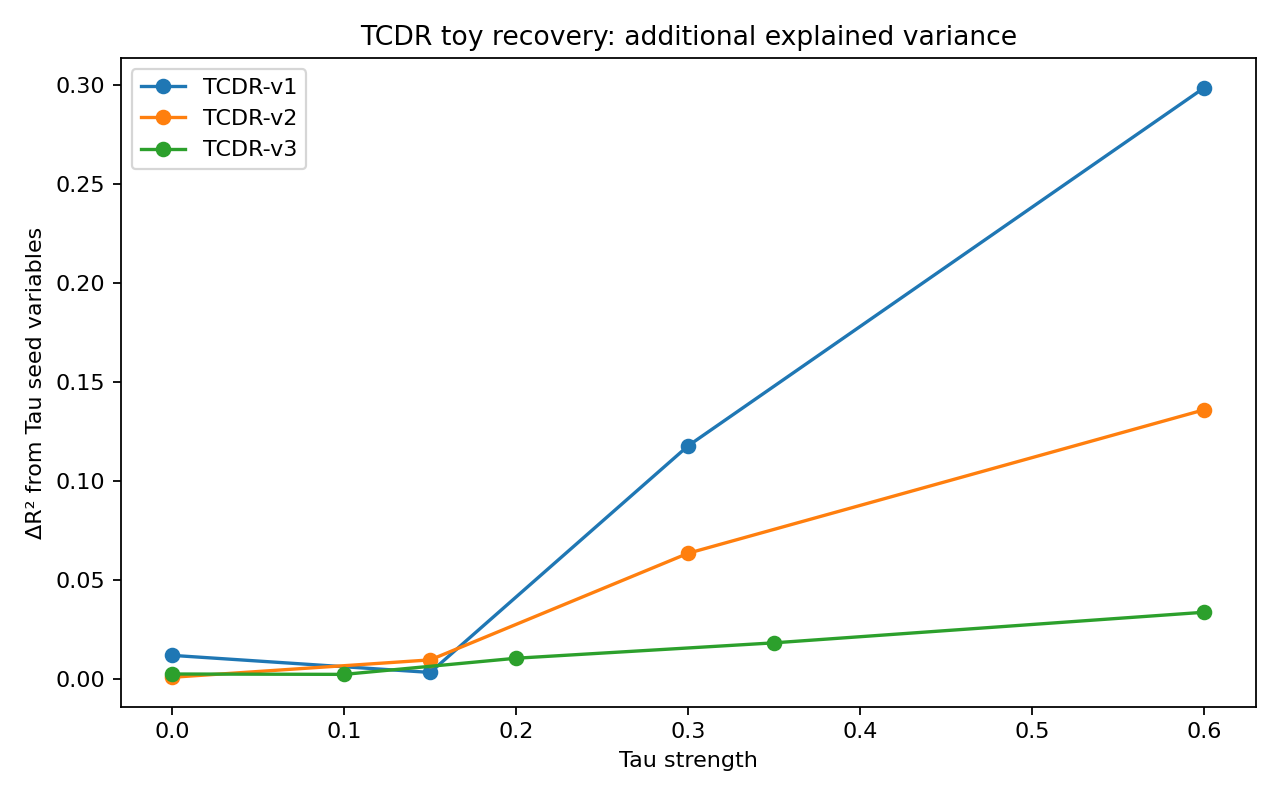
\includegraphics[width=0.82\linewidth]{figures/tcdr_delta_r2.png}
\caption{Additional explained variance from predeclared Tau seed variables in
the synthetic TCDR toys.  Stronger injected seed strength is recovered in
TCDR-v1 and TCDR-v2; TCDR-v3 is deliberately harder because it uses a
differential null/time split.}
\label{fig:delta-r2}
\end{figure}

\section{TCDR-v2: Noisy Controls}

TCDR-v2 adds halo nonlinearity, baryonic uncertainty, inclination-like error,
filament angle error, bar/disk orientation error, and survey-like directional
systematics.  This version asks whether the seed recovery collapses under
more realistic nuisance structure.  It does not.  The no-injection case
remains score 0, while \(\tau=0.30\) and \(\tau=0.60\) reach score 4 with
permutation \(p\simeq0.001996\).

\begin{figure}[H]
\centering
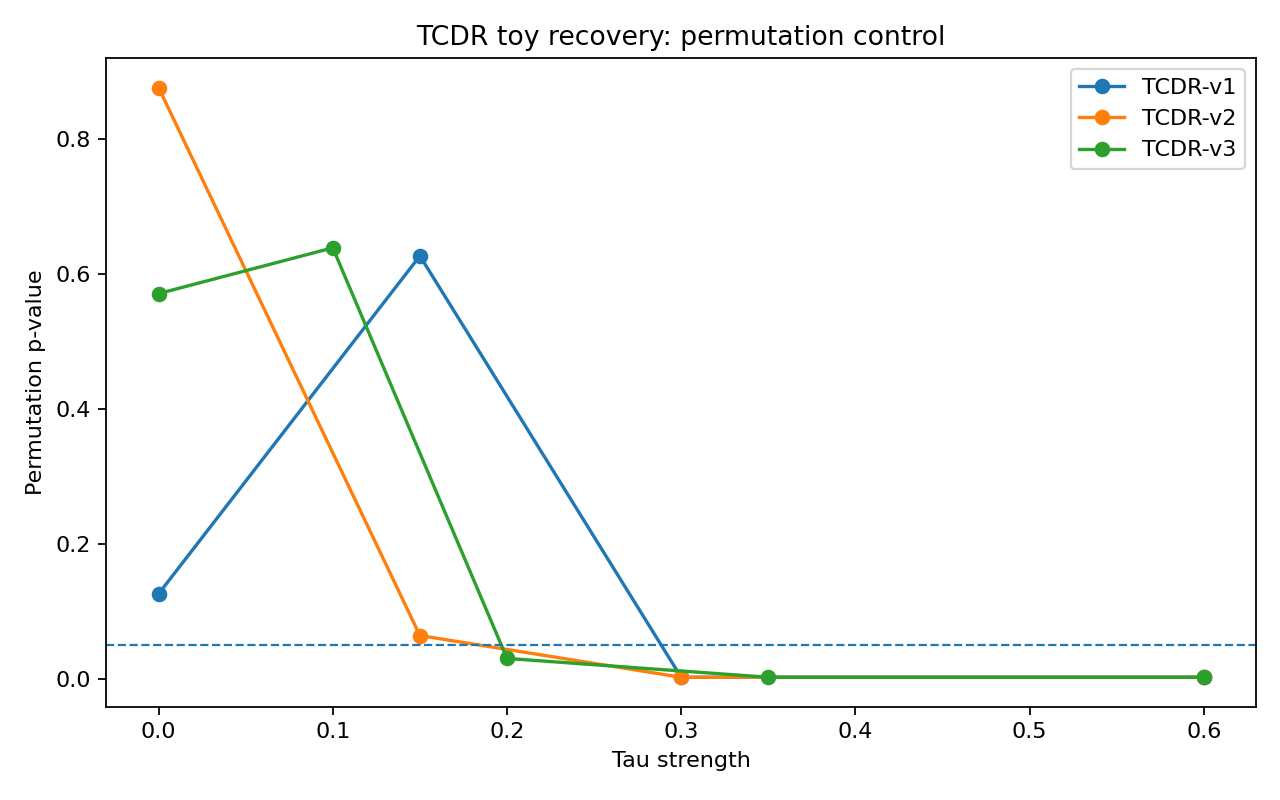
\includegraphics[width=0.82\linewidth]{figures/tcdr_pvalues.png}
\caption{Permutation control for the TCDR toys.  The horizontal line marks
\(p=0.05\).  These p-values are toy permutation statistics under the package
simulation; they are not observational p-values.}
\label{fig:pvalues}
\end{figure}

\section{TCDR-v3: Null/Time Split}

TCDR-v3 is the most Tau-Core-specific toy in the package.  It creates two
mock residual channels:
\begin{align}
  R_{\rm time} &= R_{\rm common}+0.35\,\tau P_{\tau}+\eta_{\rm time},\\
  R_{\rm null} &= R_{\rm common}+1.00\,\tau P_{\tau}+\eta_{\rm null}.
\end{align}
The tested endpoint is the differential split
\[
  \Delta_{\tau}=R_{\rm null}-R_{\rm time}.
\]
The no-injection and very weak injection runs remain score 0.  The
\(\tau=0.20\) run reaches score 2, while \(\tau=0.35\) and \(\tau=0.60\)
reach score 3.  This is weaker than the clean morphology toy, as expected,
because the split is noisier and differential.

\begin{figure}[H]
\centering
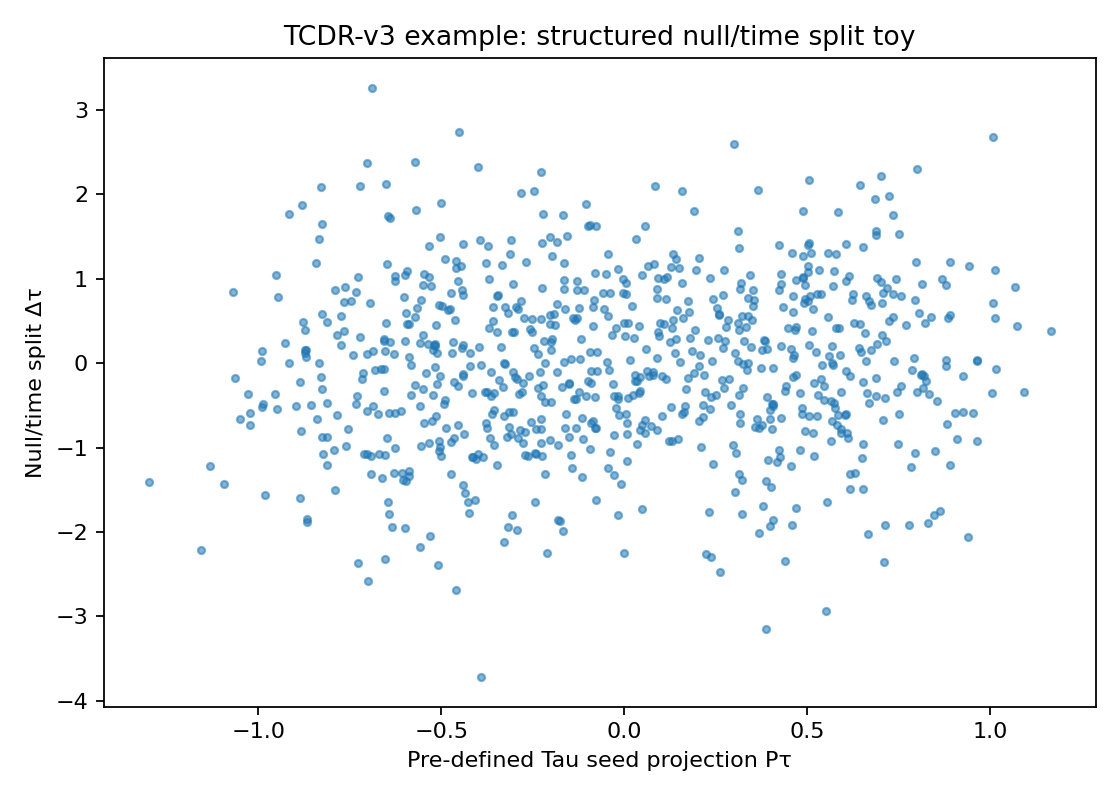
\includegraphics[width=0.80\linewidth]{figures/tcdr_v3_split_scatter.png}
\caption{TCDR-v3 example split.  The plotted relation is between the
predefined seed \(P_{\tau}\) and the toy null/time split \(\Delta_{\tau}\) for
the fixed \(\tau=0.35\) example dataset.}
\label{fig:split-scatter}
\end{figure}

\section{Numerical Summary}

\begin{table}[H]
\centering
\scriptsize
\begin{tabular}{llrrrr}
\toprule
Module & \(\tau\) & \(R^2_{\rm base}\) & \(R^2_{\tau}\) & \(\Delta R^2\) & Score\\
\midrule
TCDR-v1 & 0.00 & 0.1303 & 0.1422 & 0.0119 & 0\\
TCDR-v1 & 0.15 & 0.0757 & 0.0790 & 0.0032 & 0\\
TCDR-v1 & 0.30 & 0.0795 & 0.1973 & 0.1178 & 4\\
TCDR-v1 & 0.60 & 0.0444 & 0.3431 & 0.2987 & 5\\
TCDR-v2 & 0.00 & 0.1587 & 0.1595 & 0.0008 & 0\\
TCDR-v2 & 0.15 & 0.1781 & 0.1877 & 0.0096 & 0\\
TCDR-v2 & 0.30 & 0.1305 & 0.1940 & 0.0635 & 4\\
TCDR-v2 & 0.60 & 0.1557 & 0.2916 & 0.1360 & 4\\
TCDR-v3 & 0.00 & 0.0012 & 0.0036 & 0.0024 & 0\\
TCDR-v3 & 0.10 & 0.0135 & 0.0157 & 0.0023 & 0\\
TCDR-v3 & 0.20 & 0.0038 & 0.0142 & 0.0104 & 2\\
TCDR-v3 & 0.35 & 0.0155 & 0.0337 & 0.0182 & 3\\
TCDR-v3 & 0.60 & 0.0012 & 0.0349 & 0.0337 & 3\\
\bottomrule
\end{tabular}
\caption{Fixed-seed TCDR summary generated by the package script.  The table
is synthetic and should not be read as empirical evidence.}
\label{tab:summary}
\end{table}

\begin{figure}[H]
\centering
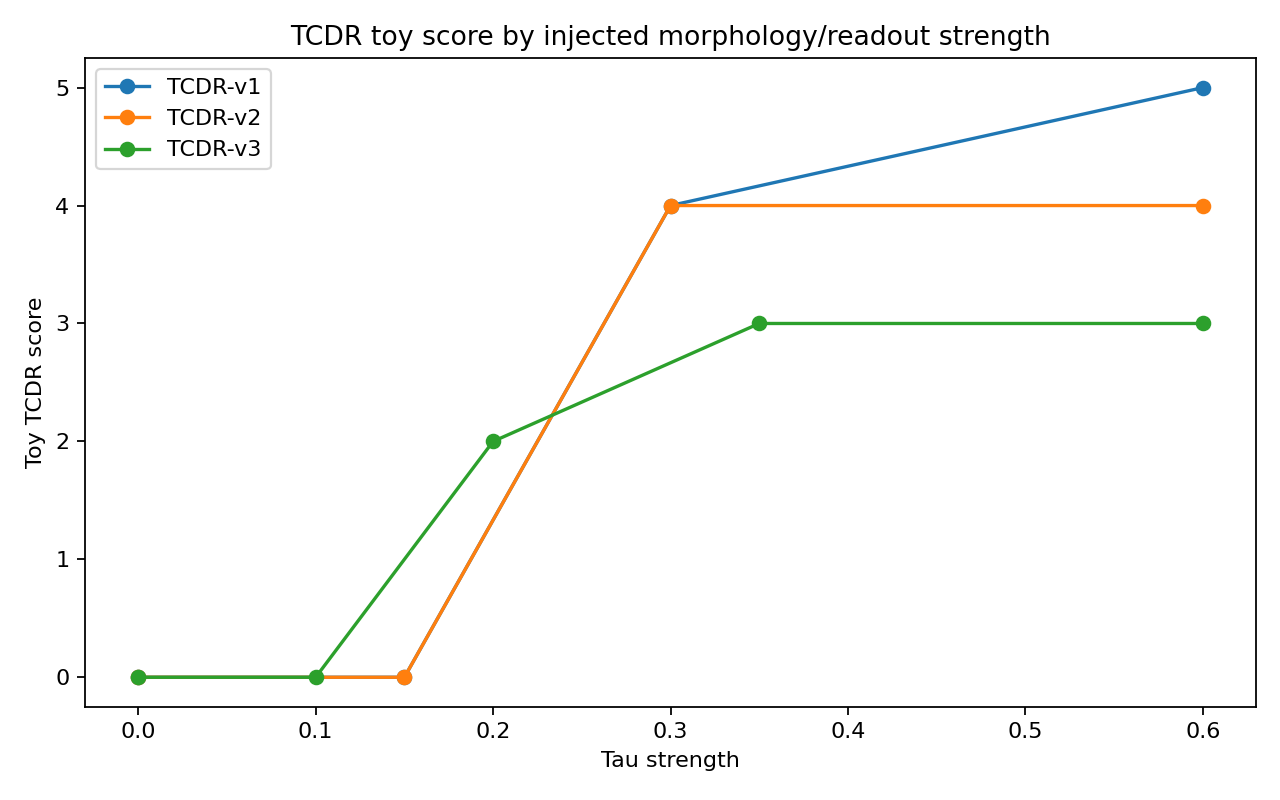
\includegraphics[width=0.82\linewidth]{figures/tcdr_score.png}
\caption{Toy TCDR score by injected morphology/readout strength.  The null
runs score zero, while stronger injections produce recoverable synthetic
signals.}
\label{fig:score}
\end{figure}

\section{Multi-Seed Robustness Replay}

The fixed-seed result is not enough by itself.  To test whether the toy result
is brittle, the package also runs a 32-seed replay on the null and
stronger-injection cases.  This is still synthetic, but it probes whether the
reported pattern depends on one random draw.

\begin{table}[H]
\centering
\scriptsize
\begin{tabular}{llrrrr}
\toprule
Module & \(\tau\) & \(n\) & Mean \(\Delta R^2\) & Pass floor & Null false positive\\
\midrule
TCDR-v1 & 0.00 & 32 & 0.0059 & 1.000 & 0.062\\
TCDR-v1 & 0.60 & 32 & 0.2514 & 1.000 & --\\
TCDR-v2 & 0.00 & 32 & 0.0037 & 1.000 & 0.031\\
TCDR-v2 & 0.60 & 32 & 0.1470 & 1.000 & --\\
TCDR-v3 & 0.00 & 32 & 0.0026 & 1.000 & 0.000\\
TCDR-v3 & 0.35 & 32 & 0.0183 & 0.563 & --\\
TCDR-v3 & 0.60 & 32 & 0.0402 & 0.969 & --\\
\bottomrule
\end{tabular}
\caption{Multi-seed replay summary.  The pass floor is the fraction passing the
predeclared toy score floor for that case.  For null rows, the relevant
quantity is the false-positive rate, not the pass floor, because the expected
score floor is zero.}
\label{tab:multiseed}
\end{table}

\begin{figure}[H]
\centering
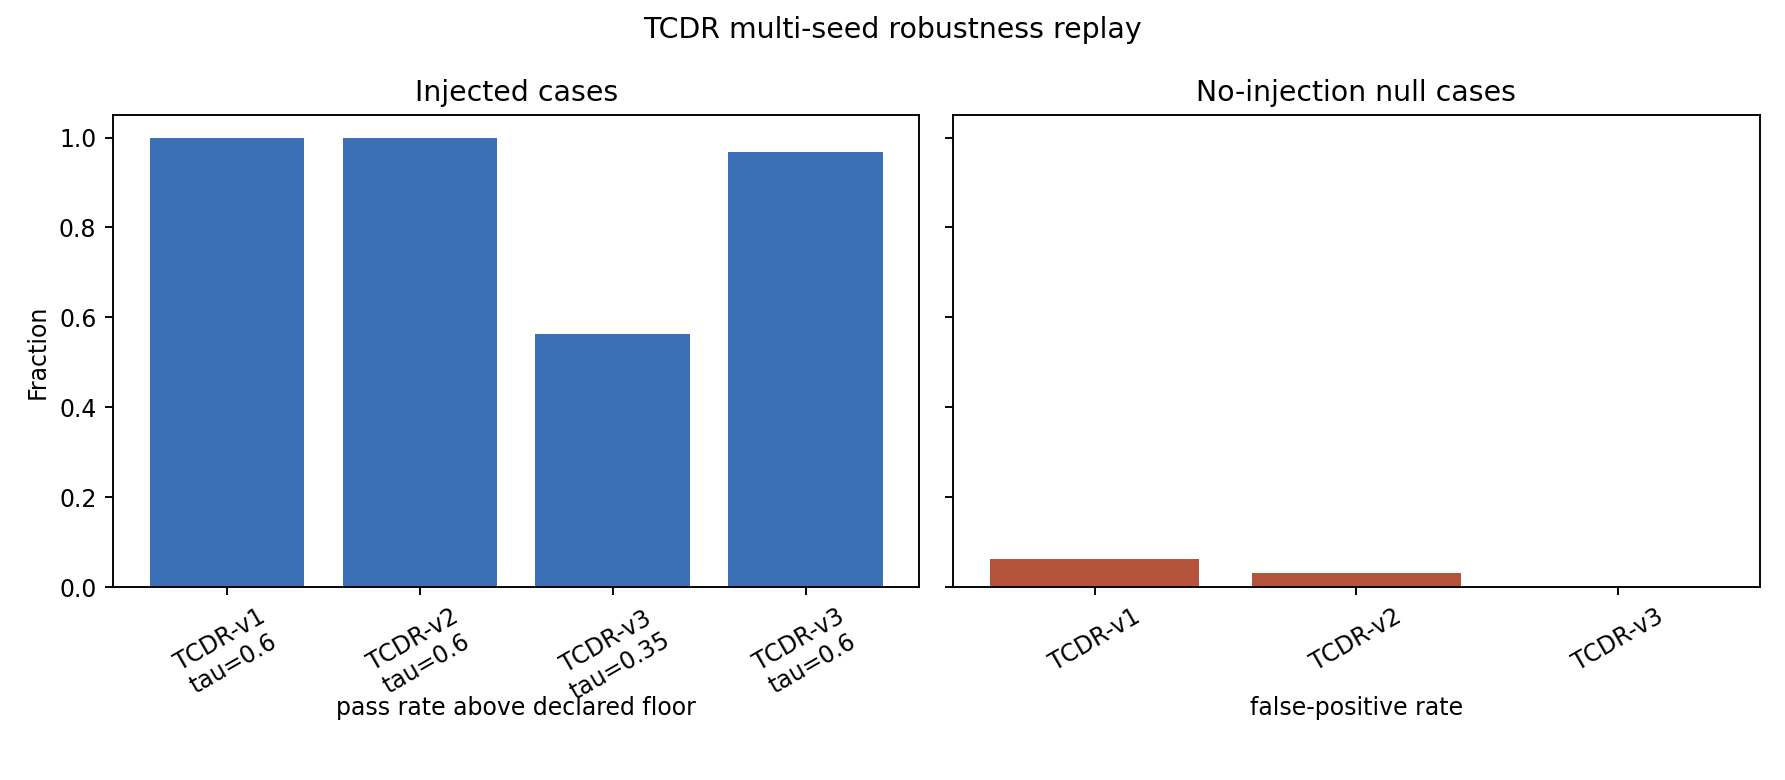
\includegraphics[width=0.84\linewidth]{figures/tcdr_multiseed_passrate.png}
\caption{Multi-seed replay pass fractions.  TCDR-v1 and TCDR-v2 strong
injections are stable in this toy.  TCDR-v3 at \(\tau=0.35\) is only partially
stable, while the stronger split case is much more robust.}
\label{fig:multiseed}
\end{figure}

The threshold sweep supports the same cautious reading.  For example, at
\(p\le 0.01\) and \(\Delta R^2\ge 0.015\), the injected-positive recovery
fraction is \(0.883\), while the null false-positive fraction is \(0.000\).
At the looser \(p\le 0.05\), \(\Delta R^2\ge 0.010\) setting, recovery rises
to \(0.953\), but the null false-positive fraction becomes \(0.031\).  These
numbers are not discovery statistics; they are robustness checks for the
synthetic protocol thresholds.

\begin{figure}[H]
\centering
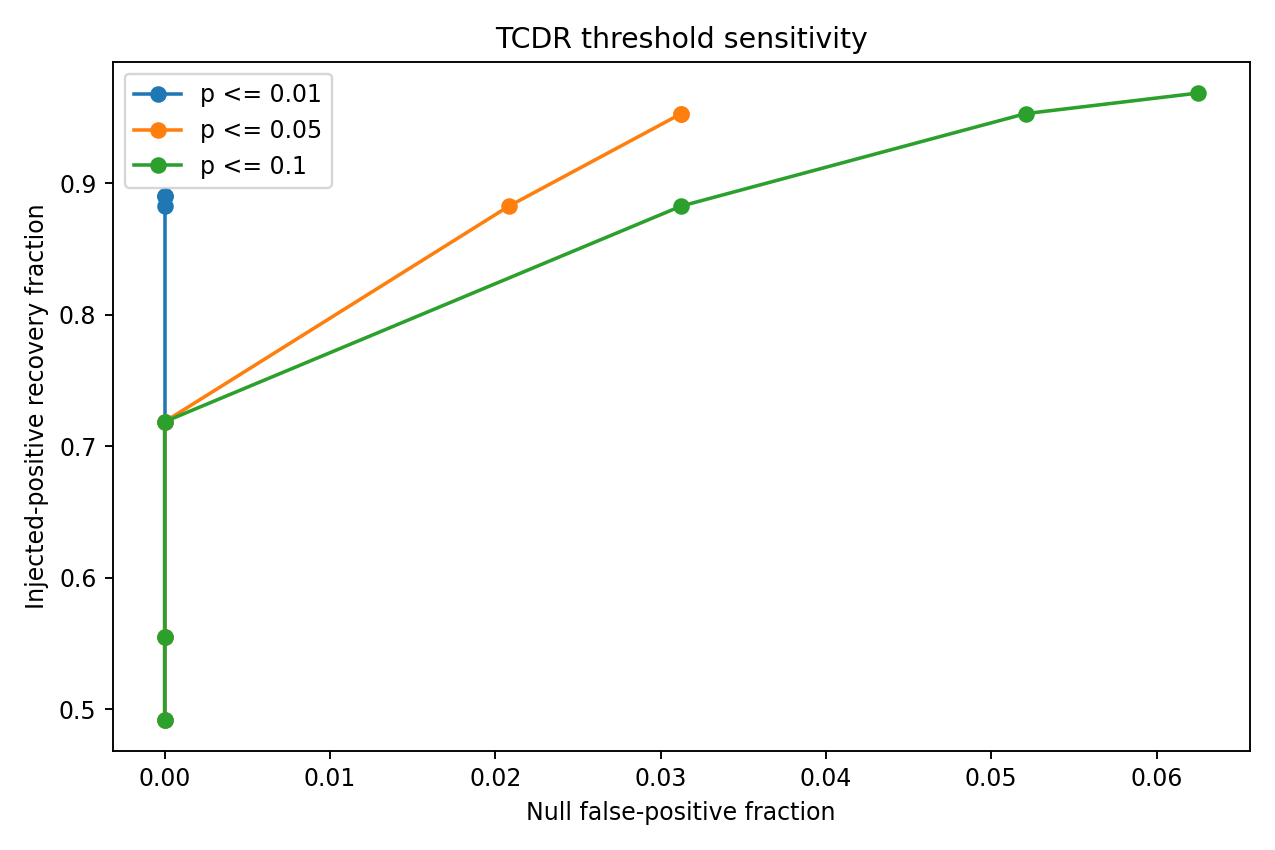
\includegraphics[width=0.78\linewidth]{figures/tcdr_threshold_sensitivity.png}
\caption{Threshold sensitivity for the multi-seed replay.  The plot reports
the tradeoff between injected-positive recovery and null false positives under
different \(p\)-value and \(\Delta R^2\) thresholds.}
\label{fig:threshold-sensitivity}
\end{figure}

\section{Blinded Synthetic Injection Challenge}

The next stress test is closer to a miniature challenge problem.  The script
generates 26 synthetic challenge rows: 8 no-injection null cases and 18
injected cases spanning weak, medium, and stronger seed strengths.  The
scoring stage does not use the hidden injection label.  It uses a frozen rule:
\[
  p \le 0.05,\qquad
  \Delta R^2_{\rm correct}\ge 0.020,\qquad
  \Delta R^2_{\rm correct}-\Delta R^2_{\rm wrong}\ge 0.010.
\]
The wrong-seed model uses plausible morphology/environment columns with
incorrect source-side alignment.  This is meant to test whether the correct
source seed beats a wrong-family seed, not merely whether any extra columns
improve the regression.

\begin{table}[H]
\centering
\scriptsize
\begin{tabular}{L{0.42\linewidth}r}
\toprule
Quantity & Value\\
\midrule
Number of challenge mocks & 26\\
Hidden injected mocks & 18\\
No-injection null mocks & 8\\
True positives & 12\\
False positives & 0\\
True negatives & 8\\
False negatives & 6\\
Accuracy & 0.769\\
True-positive rate & 0.667\\
False-positive rate & 0.000\\
Median correct-seed \(\Delta R^2\) & 0.0100\\
Median wrong-seed \(\Delta R^2\) & 0.0048\\
\bottomrule
\end{tabular}
\caption{Blind synthetic injection challenge.  The outcome is deliberately
conservative: the classifier protects null cases at the price of missing
weak/borderline injected cases.}
\label{tab:blind-challenge}
\end{table}

\begin{figure}[H]
\centering
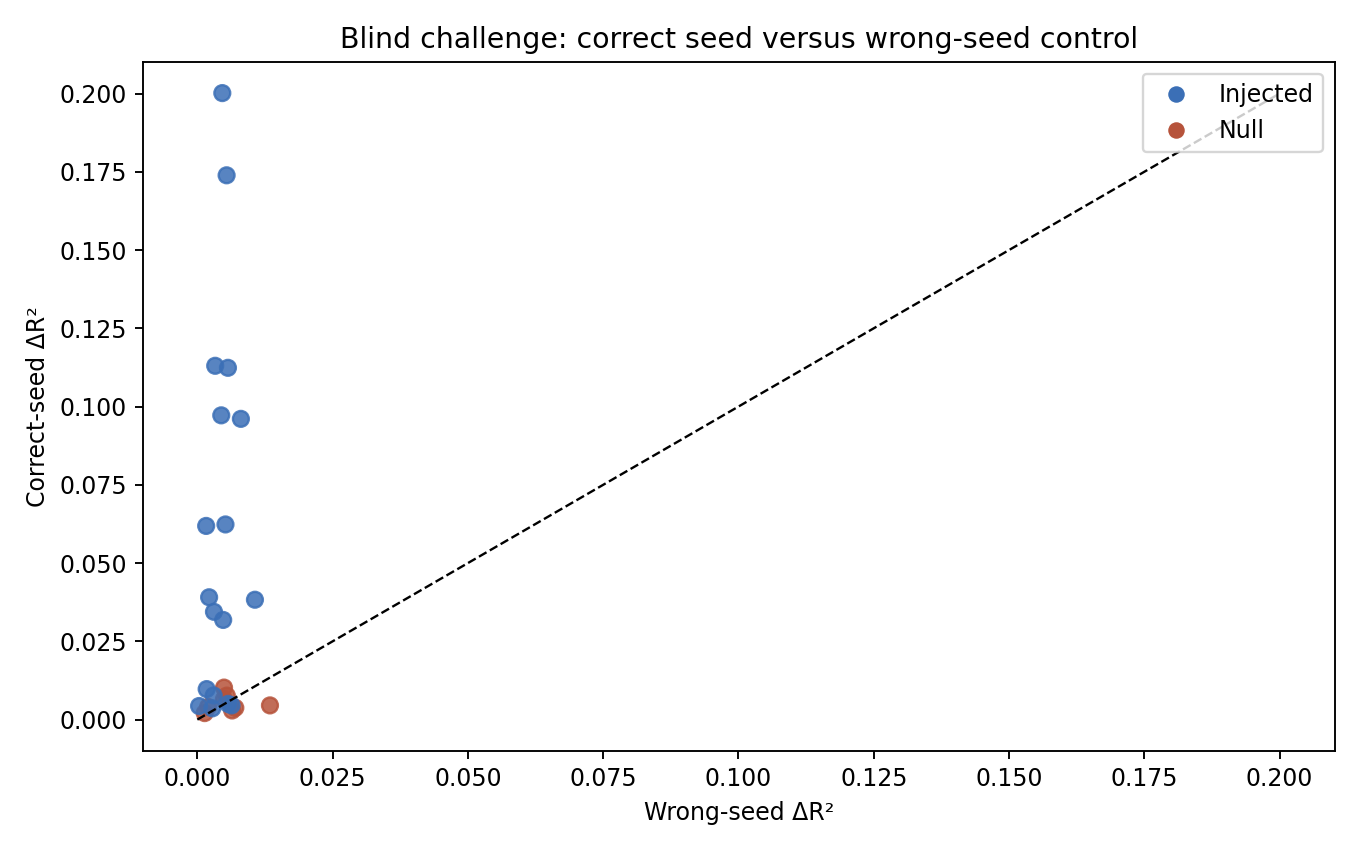
\includegraphics[width=0.78\linewidth]{figures/tcdr_blind_correct_vs_wrong.png}
\caption{Correct-seed versus wrong-seed \(\Delta R^2\) in the blind challenge.
Injected cases are blue and null cases are red.  Points above the dashed line
favor the correct source-side seed over the wrong-seed control.}
\label{fig:blind-correct-wrong}
\end{figure}

\begin{figure}[H]
\centering
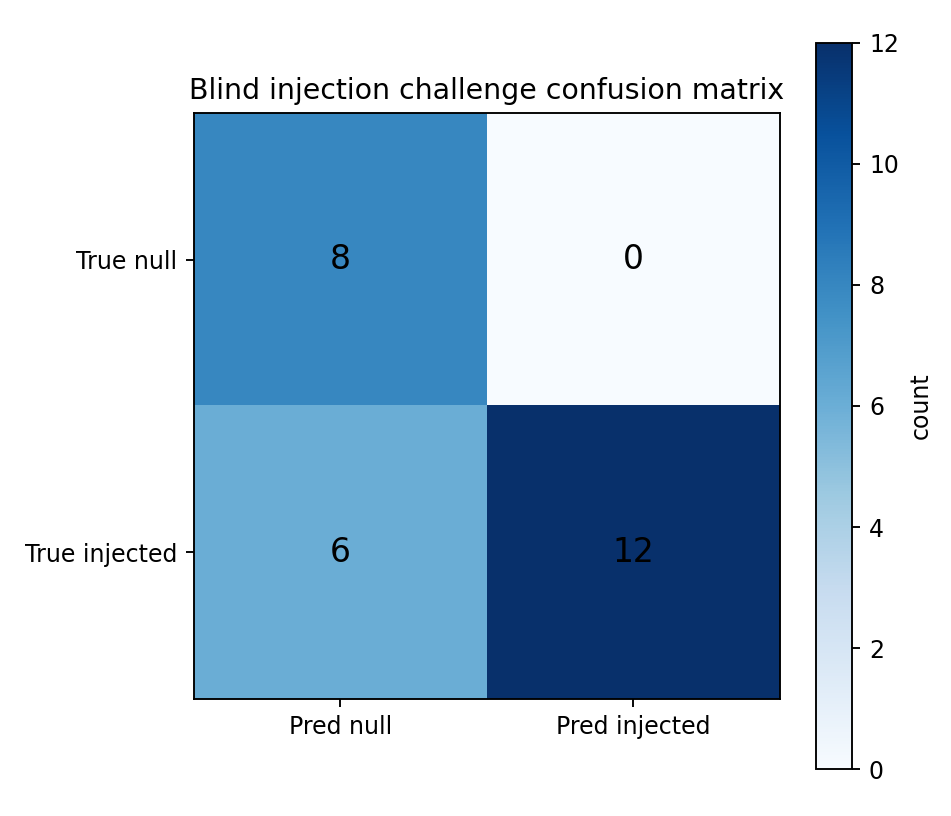
\includegraphics[width=0.56\linewidth]{figures/tcdr_blind_confusion.png}
\caption{Blind challenge confusion matrix.  The protocol produces no false
positives in this synthetic challenge, but it misses 6 weak or borderline
injections.  This should be read as controlled specificity, not universal
sensitivity.}
\label{fig:blind-confusion}
\end{figure}

\section{Realistic-Mock Nuisance Stress Test}

The v0.3 blind challenge is still too clean to mimic the way false residual
structure can appear in survey-facing work.  The v0.4 stress test therefore
adds nuisance layers that are deliberately capable of producing misleading
structure:
\begin{itemize}
  \item a shared sky-mask variable;
  \item foreground-like contamination;
  \item source-selection bias;
  \item line-of-sight orientation structure;
  \item a wrong-seed morphology/environment control;
  \item an orientation-only control;
  \item a random-control channel.
\end{itemize}
The base model receives the survey-mask, foreground, selection, sky-position,
halo, baryonic, inclination-like, shear-calibration-like, and local-density
variables.  The candidate model then adds only the predeclared source seed
columns.  The frozen positive rule is:
\[
  p \le 0.05,\qquad
  \Delta R^2_{\rm candidate}\ge 0.020,\qquad
  \Delta R^2_{\rm candidate}-\max(\Delta R^2_{\rm controls})\ge 0.008 .
\]
This is a realistic nuisance robustness check, not a real survey analysis.
The hidden injection labels are used only after scoring to build the confusion
matrix.

\begin{table}[H]
\centering
\scriptsize
\begin{tabular}{L{0.46\linewidth}r}
\toprule
Quantity & Value\\
\midrule
Number of realistic-mock challenges & 32\\
Hidden injected mocks & 22\\
No-injection null mocks & 10\\
True positives & 11\\
False positives & 0\\
True negatives & 10\\
False negatives & 11\\
Accuracy & 0.656\\
True-positive rate & 0.500\\
False-positive rate & 0.000\\
Median candidate \(\Delta R^2\) & 0.0079\\
Median strongest-control \(\Delta R^2\) & 0.0085\\
Median candidate-minus-control margin & -0.0012\\
\bottomrule
\end{tabular}
\caption{Realistic-mock nuisance stress test.  The classifier is intentionally
specificity-first: it rejects every null case in this synthetic run, but misses
half of the injected cases.  This is a useful caution, not a validation
result.}
\label{tab:realistic-mock}
\end{table}

\begin{figure}[H]
\centering
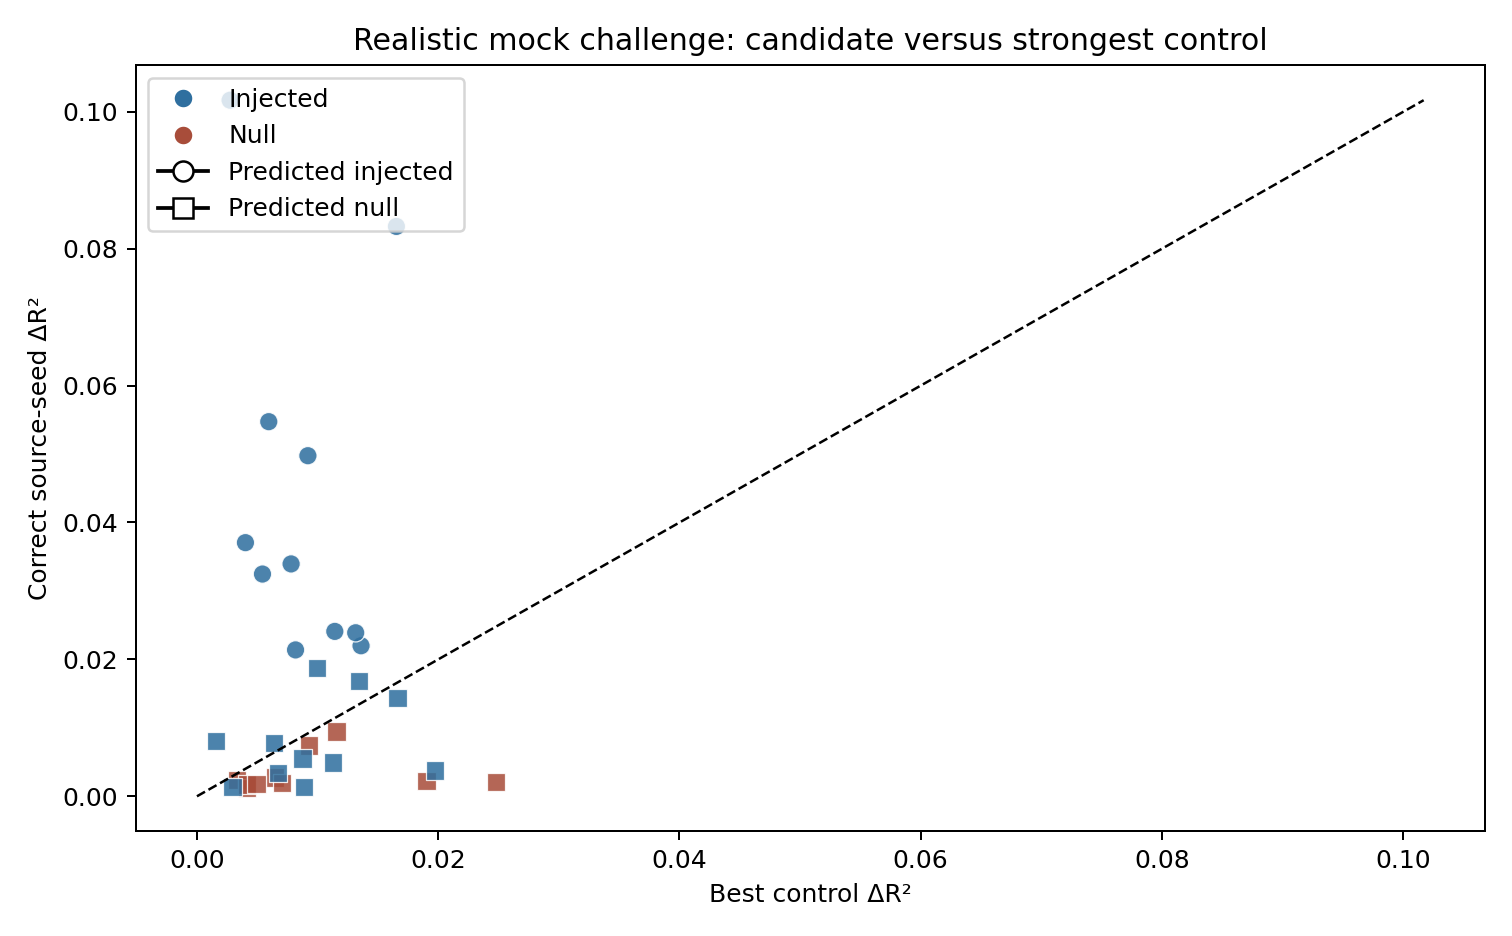
\includegraphics[width=0.80\linewidth]{figures/tcdr_realistic_candidate_vs_controls.png}
\caption{Candidate seed versus strongest control in the realistic-mock stress
test.  The strongest control is the maximum of wrong-seed, orientation-only,
and random-control \(\Delta R^2\).  Points above the dashed line favor the
candidate source seed, but the frozen classifier also requires the \(p\)-value,
\(\Delta R^2\), and margin cuts.}
\label{fig:realistic-candidate-controls}
\end{figure}

\begin{figure}[H]
\centering
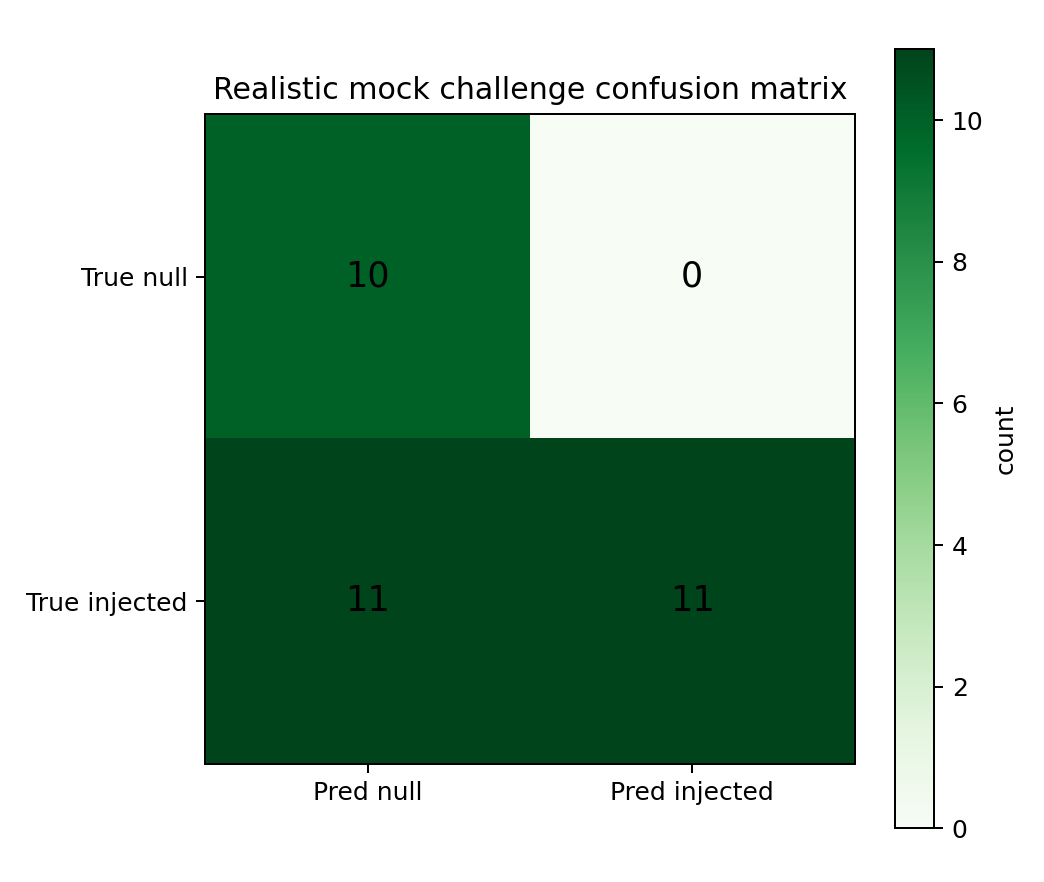
\includegraphics[width=0.56\linewidth]{figures/tcdr_realistic_confusion.png}
\caption{Confusion matrix for the realistic-mock stress test.  The zero
false-positive result is encouraging for specificity, while the 11 false
negatives show that weak and borderline signals are not reliably recovered
under harder nuisance structure.}
\label{fig:realistic-confusion}
\end{figure}

\begin{figure}[H]
\centering
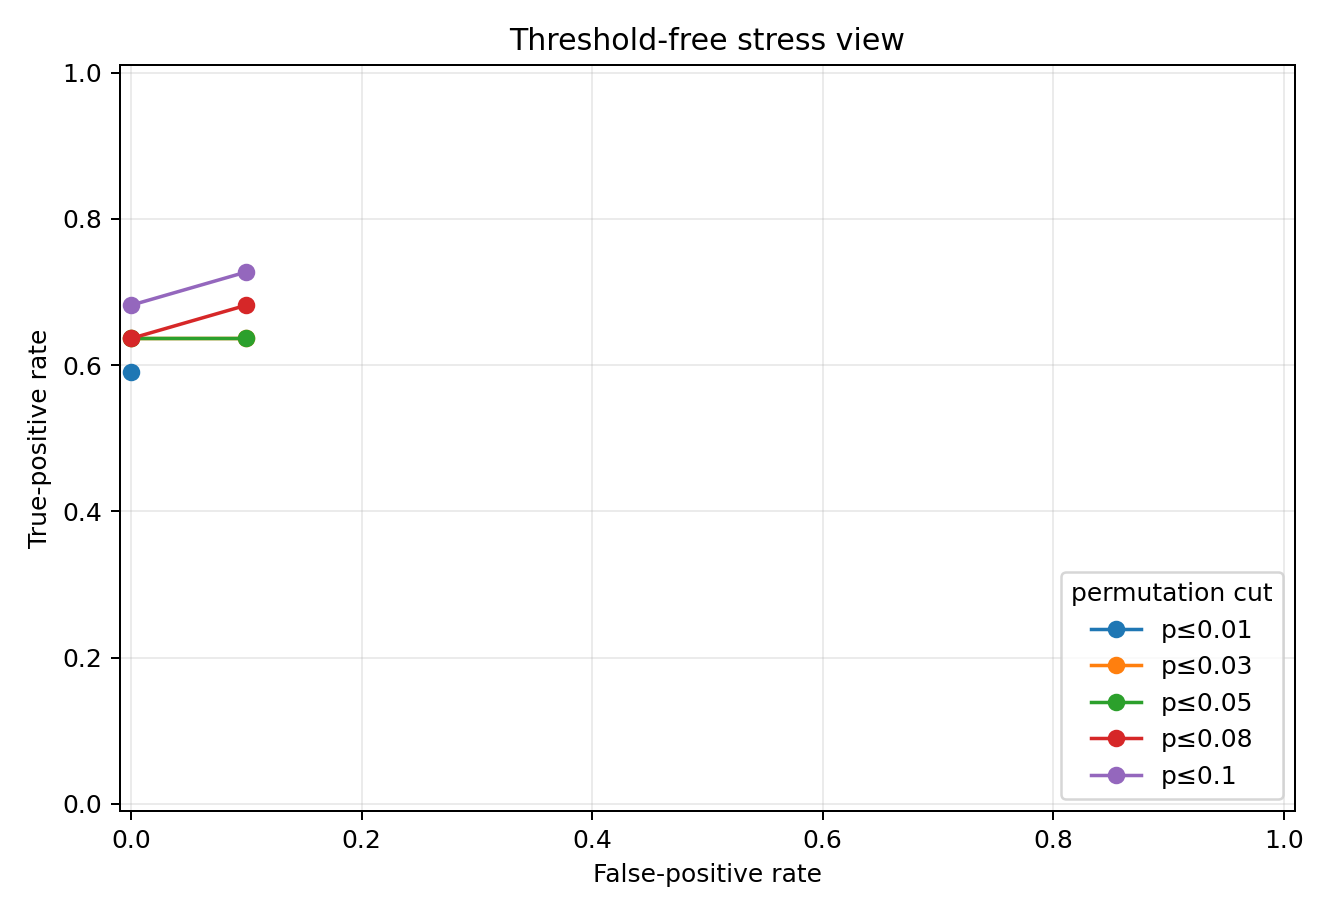
\includegraphics[width=0.76\linewidth]{figures/tcdr_realistic_threshold_curve.png}
\caption{Threshold-free stress view for the realistic-mock challenge.  The
curves show the tradeoff between true-positive and false-positive rate as the
\(\Delta R^2\), margin, and permutation thresholds vary.  This figure is meant
to prevent over-reading a single frozen threshold.}
\label{fig:realistic-threshold}
\end{figure}

\section{TCDR-v4 Real-Data Source Manifest}

The move from synthetic toys to real data must begin with source-role
separation, not with endpoint fitting.  The repository therefore includes a
machine-generated manifest:
\begin{center}
\texttt{data/source\_manifests/tcdr\_v4\_real\_data\_source\_manifest\_v0\_1.csv}.
\end{center}
It is generated by:
\begin{center}
\texttt{python scripts/build\_tcdr\_v4\_real\_data\_manifest.py}.
\end{center}

The manifest records public source candidates and their allowed TCDR roles.
The most important rule is that endpoint dynamics data may score a frozen
candidate, but may not choose or rescue the source-side morphology label.  In
particular, SPARC rotation-curve and mass-model products are endpoint/baseline
data \cite{SPARCWebsite}.  S4G/IRSA products and Galaxy Zoo morphology
catalogues are source-side morphology routes \cite{S4GIRSA,GalaxyZooData}.
EDD/Cosmicflows-style distance and velocity products can provide distance or
environment controls, but any amplitude use must be frozen before scoring
\cite{EDDWebsite}.

For local preflight only, the repository also provides an optional downloader:
\begin{center}
\texttt{python scripts/download\_tcdr\_v4\_sparc\_endpoint.py --out-dir data/external/sparc\_preflight}.
\end{center}
The downloaded files are ignored by git and are endpoint/baseline inputs only.
They must not be used for source-label selection.

After the SPARC sample table is available locally, the source-freeze queue is
built by:
\begin{center}
\texttt{python scripts/build\_tcdr\_v4\_sparc\_source\_freeze\_queue.py}.
\end{center}
The script reads SPARC sample metadata only and intentionally excludes
\(V_{\rm flat}\) and rotation-curve endpoint values.  Its current output
contains 175 SPARC objects:
\begin{align*}
  66 &\quad {\rm P0\_SOURCE\_REVIEW},\\
  60 &\quad {\rm P1\_SOURCE\_REVIEW},\\
  49 &\quad {\rm P2\_SOURCE\_REVIEW}.
\end{align*}
The priority labels are source-review logistics, not evidence levels.  They
rank objects for later S4G/Galaxy Zoo morphology lookup using quality,
inclination, HI-extent availability, and catalogue-name queryability.  No
endpoint residual is inspected.

The first S4G lookup uses the IRSA TAP table \texttt{s4gcat} and source-side
columns such as optical type, bar/ring flags, IR position angle, ellipticity,
concentration, and stellar-mass proxy fields.  For the 66 P0 objects, the
current name-based lookup returns:
\begin{align*}
  32 &\quad {\rm S4G\ matched\ by\ name},\\
  34 &\quad {\rm not\ found\ by\ name}.
\end{align*}
The unmatched objects are not failures; they require alias review or a
different source-side morphology route.  The lookup artifact is
\path{data/source_manifests/tcdr_v4_p0_s4g_lookup_v0_1.csv}.

A second resolver pass uses SIMBAD coordinates for the 34 name-unmatched
objects and performs a 1 arcmin nearest-neighbour cross-match against S4G
positions.  This adds:
\begin{align*}
  11 &\quad {\rm S4G\ coordinate\ matched},\\
  23 &\quad {\rm still\ outside\ the\ S4G\ coordinate\ match\ radius}.
\end{align*}
Thus the present P0 S4G source-side coverage is 43/66 before endpoint scoring.
This remains an availability ledger only; it is not a residual or rotation
curve result.  The coordinate artifact is
\path{data/source_manifests/tcdr_v4_p0_s4g_coordinate_lookup_v0_1.csv}.

For the remaining 23 non-S4G P0 objects, a SIMBAD fallback pass resolves all
23 object identities and provides morphology-type fields for 22:
\begin{align*}
  23 &\quad {\rm SIMBAD\ resolved},\\
  22 &\quad {\rm SIMBAD\ morphology\ type\ available},\\
   1 &\quad {\rm SIMBAD\ identity\ only}.
\end{align*}
This fallback is deliberately lower in the source hierarchy than S4G: it
records catalogue identity, object type, morphology type, morphology bibcode,
and aliases, but it is not a homogeneous infrared morphology measurement.  It
is retained as a source-side fallback ledger only.  The artifact is
\path{data/source_manifests/tcdr_v4_p0_simbad_fallback_lookup_v0_1.csv}.

Combining the three source ledgers gives the first freeze-ready P0 source-tier
manifest:
\begin{align*}
  32 &\quad {\rm S4G\_STRONG},\\
  11 &\quad {\rm S4G\_COORD\_RESCUE},\\
  22 &\quad {\rm SIMBAD\_FALLBACK},\\
   1 &\quad {\rm SIMBAD\_IDENTITY\_ONLY}.
\end{align*}
Equivalently, all 66 P0 objects have an identity tier, 65 have some
source-side morphology type, and 43 have homogeneous S4G structural morphology.
These tiers are source-quality classes only.  They are not fit classes,
endpoint scores, or claims that the corresponding readout family will improve
a rotation curve.  The artifact is
\path{data/source_manifests/tcdr_v4_p0_source_tier_manifest_v0_1.csv}.

The first endpoint-blind family freeze maps these source tiers into candidate
readout families using only source-side morphology rules:
\begin{align*}
  30 &\quad {\rm K\_BARRED\_M2},\\
  14 &\quad {\rm K\_EXPONENTIAL\_SPIRAL\_DISK},\\
  10 &\quad {\rm K\_RING\_RESONANCE},\\
   6 &\quad {\rm K\_DIFFUSE\_LATE\_DISK},\\
   5 &\quad {\rm K\_COMPACT\_EARLY\_DISK},\\
   1 &\quad {\rm K\_UNFREEZABLE\_IDENTITY\_ONLY}.
\end{align*}
The selection grammar is deliberately simple: ring flags dominate ring
families; bar flags or barred morphology select the barred family; late or
irregular morphology selects diffuse late disks; early/S0 morphology selects
compact early disks; otherwise the default is an exponential spiral disk.
High ellipticity or high inclination is recorded only as a projection caveat,
not as an endpoint correction.  The family-freeze artifact is
\path{data/source_manifests/tcdr_v4_p0_source_family_freeze_v0_1.csv}.

The next source-side artifact is a first homogeneous-S4G pilot holdout
manifest.  It is generated from the already frozen family manifest by:
\begin{center}
\texttt{python scripts/build\_tcdr\_v4\_p0\_pilot\_holdout\_manifest.py}.
\end{center}
The selection is deterministic and endpoint-blind: within each homogeneous
S4G source family, the script selects up to two objects, preferring entries
without projection caveats and then sorting by galaxy name, while leaving at
least one train object in every selected homogeneous family.  This calibration
aware guard prevents small families from being exhausted into holdout before
any family-level amplitude or control can be estimated.  The current
artifact contains:
\begin{align*}
   7 &\quad {\rm PILOT\_HOLDOUT},\\
  36 &\quad {\rm PILOT\_TRAIN\_POOL},\\
  23 &\quad {\rm NON\_HOMOGENEOUS\_SOURCE\_TIER}.
\end{align*}
The holdout family counts are:
\begin{align*}
  2 &\quad {\rm K\_BARRED\_M2},\\
  1 &\quad {\rm K\_DIFFUSE\_LATE\_DISK},\\
  2 &\quad {\rm K\_EXPONENTIAL\_SPIRAL\_DISK},\\
  2 &\quad {\rm K\_RING\_RESONANCE}.
\end{align*}
This is a scoring-preparation ledger only.  It does not inspect rotation
residuals, fit amplitudes, compare baselines, or claim that the matched family
improves any galaxy.  The CSV and JSON artifacts are stored in the repository
source-manifest directory with the pilot-holdout prefix.

Finally, the current local preflight checks endpoint availability for the
frozen holdout without committing the endpoint curves.  The script
\begin{center}
\texttt{python scripts/build\_tcdr\_v4\_p0\_holdout\_endpoint\_packet.py}
\end{center}
requires the optional local SPARC preflight files and writes two classes of
output.  The committed readiness manifest records only availability and coarse
curve metadata:
\begin{align*}
  7   &\quad {\rm holdout\ objects\ with\ endpoint\ rows},\\
 215  &\quad {\rm total\ local\ rotation\ points}.
\end{align*}
The actual SPARC endpoint curve packet is written only under
\path{data/external/}, which is ignored by git.  The frozen carrier policy is
\({\rm disk}\ M/L=0.5\) and \({\rm bulge}\ M/L=0.7\), with no amplitude fit.
This is endpoint-readiness only: no score, residual comparison, baseline
ranking, or physical claim is made at this stage.

A separate optional local scoring preflight is provided only as a diagnostic.
It fits non-negative family amplitudes on the \({\rm PILOT\_TRAIN\_POOL}\)
and scores only the frozen holdout.  Families with fewer than two train
galaxies are marked calibration-blocked and are not allowed to act as matched
endpoint results or wrong-family controls.  This rule is deliberately
conservative: an under-supported source family may remain endpoint-ready for
future data, but it is not treated as a calibrated control in the present
preflight.

The current author-local scoring pass uses a train-pool-only
specificity-first v4 kernel policy:
\[
{\rm train\_pool\_only\_specificity\_first\_v4\_penalty\_1p5\_no\_holdout\_shape\_tuning}.
\]
In that diagnostic run, six holdout galaxies are scoreable and one diffuse
late-disk holdout is calibration-blocked.  The matched family improves the
frozen baryonic carrier in \(6/6\) scoreable cases, beats the calibrated
wrong-family mean in \(3/6\), and beats the best calibrated wrong family in
\(2/6\).  The median wrong-family-mean minus matched weighted RMSE is
\(-0.074\,{\rm km\,s^{-1}}\), while the median matched minus baryonic-carrier
weighted RMSE is \(-0.392\,{\rm km\,s^{-1}}\).  This is a useful
kernel-development diagnostic, not a validation result: the present
source-family kernels are still too primitive for robust endpoint-level
family separation.

The companion kernel-specificity diagnosis makes the weakness more precise.
Among the scoreable holdout objects, the calibrated wrong-family winners are
not arbitrary: the ordinary exponential-disk kernel is the best calibrated
family for both barred holdout objects and for both ring/resonance holdout
objects where the matched family is not best.  Thus the present failure mode
is not a request to increase amplitudes after seeing the endpoint curves.  It
is a source-side requirement: barred systems need source-native bar length,
strength, phase/orientation, and radial support; ring systems need
source-native ring radius, width, and resonance/onset class; diffuse late
disks need additional H I/low-surface-brightness train support before they can
be scored.  The diagnostic script therefore records missing source-native
coordinates rather than promoting a fitted endpoint result.

To make that requirement reproducible, the public source package now includes
an endpoint-blind source-native coordinate audit generated by:
\begin{center}
\path{python scripts/build_tcdr_v4_p0_source_native_kernel_coordinate_audit.py}.
\end{center}
Across the 66 P0 objects, the audit records:
\[
\begin{array}{rl}
30 &: {\rm barred\ objects\ requiring\ bar\ decomposition},\\
10 &: {\rm ring/resonance\ objects\ requiring\ ring\ decomposition},\\
14 &: {\rm exponential\ disks\ with\ partial\ disk/H\,I\ proxy\ coordinates},\\
6  &: {\rm diffuse\ late\ disks\ requiring\ more\ train\ support},\\
5  &: {\rm compact\ early\ disks\ outside\ the\ first\ homogeneous\ S4G\ pilot},\\
1  &: {\rm identity-only\ object\ not\ kernel-freeze\ ready}.
\end{array}
\]
This audit does not read rotation residuals, endpoint scores, or fitted
improvement margins.  Its purpose is to prevent the current binary
bar/ring/disk labels from being mistaken for source-native kernel coordinates.

The next source-route artifact asks whether the missing bar/ring coordinates
are already available in machine-readable public catalogues.  It queries the
S4G Pipeline 4 multi-component decomposition catalogue
\cite{Salo2015S4GPipeline4} and the S4G morphological feature catalogue
\cite{HerreraEndoqui2015S4GFeatures} through VizieR, using:
\begin{center}
\path{python scripts/build_tcdr_v4_p0_bar_ring_decomposition_source_route.py}.
\end{center}
Across the same 66 P0 objects, this source-route pass finds 31 objects with
Pipeline 4 decomposition rows, 21 with feature-catalogue rows, and 16 with
spiral pitch-angle rows.  Within the frozen family labels, 12 barred objects
already have source-native bar features, 4 ring/resonance objects have
source-native ring features, and 2 exponential spiral disks have source-native
spiral pitch information.  The remaining barred/ring cases are still
source-proxy cases requiring additional decomposition review.  This is not
endpoint validation; it is a reproducible source-acquisition route for the
next kernel-freeze iteration.

The corresponding endpoint-blind coordinate-freeze artifact is generated by:
\begin{center}
\path{python scripts/build_tcdr_v4_p0_source_native_kernel_coordinate_freeze.py}.
\end{center}
It converts available S4G bar/ring angular radii into physical source
coordinates using source-side sample distances and disk scales, while leaving
uncovered objects on the proxy fallback.  The frozen v0.1 rule sets the bar
kernel center to the S4G bar radius when available, sets the ring kernel
center to the S4G ring radius when available, records spiral pitch information
without using it to tune endpoint curves, and records all remaining objects as
source-proxy fallbacks.  The current freeze contains 12
source-native bar-radius objects, 4 source-native ring-radius objects, 2
spiral-pitch-recorded disk objects, and 48 source-proxy fallback objects.

An optional local endpoint replay using this coordinate-freeze rule improves
the median matched-minus-baryonic-carrier weighted RMSE margin from
\(-0.392\) to \(-0.682\,{\rm km\,s^{-1}}\), but it does not close the
family-specific endpoint gate: matched families still beat the calibrated
wrong-family mean in only \(3/6\) scoreable holdout cases and the best
calibrated wrong family in \(2/6\).  This is a useful diagnostic rather than
a validation result.  The interpretation is that source-native coordinates
help several matched objects, but mixed or multi-component galaxies can also
activate wrong-family controls unless the next rule separates components on
the source side before endpoint scoring.

The next committed source-side audit in this version therefore records
component coexistence explicitly:
\begin{center}
\path{python scripts/build_tcdr_v4_p0_source_native_component_mixture_audit.py}.
\end{center}
It uses the same S4G source-route and coordinate-freeze artifacts and does not
read endpoint curves.  Across the 66 P0 objects it finds 17
source-native mixed/multicomponent cases, 42 objects with no source-native
bar/ring/spiral component in the current S4G route, 4 single
primary-component cases, and 3 single secondary-component-only cases.  In the
7-object holdout, 3 galaxies are already mixed at source level:
NGC1090 carries bar, ring, and spiral components; NGC5033 carries ring and
spiral components; and NGC3198 carries bar, ring, and spiral components.  This
does not make wrong-family controls ``correct''.  It means that, for mixed
objects, a wrong-family control can be a source-visible secondary-component
control rather than a pure false label.  The next fair endpoint test should
therefore compare source-frozen mixed-component kernels against pure-family
and shuffled-component controls.

We therefore freeze the first mixed-component kernel rule as a separate
endpoint-blind artifact:
\begin{center}
\path{python scripts/build_tcdr_v4_p0_source_native_mixed_component_kernel_freeze.py}.
\end{center}
It assigns primary component weight \(0.5\) and lets source-visible secondary
components share the remaining \(0.5\) when multiple source-native components
are present.  Single-component cases receive weight \(1.0\), and objects
without source-native bar/ring/spiral support remain family-proxy fallbacks.
The current freeze contains 17 mixed source-native component kernels, 7
single-component kernels, and 42 fallback family-proxy kernels.  This artifact
is still source-side only: it freezes a later endpoint test rule, not a fitted
endpoint result.

The matching null-control artifact is also frozen before endpoint scoring:
\begin{center}
\path{scripts/build_tcdr_v4_p0_source_native_shuffled_component_nulls.py}.
\end{center}
It creates 64 deterministic source-side shuffles using seed 19019.  The shuffle
preserves component weights within each pilot role while breaking the
galaxy/component assignment.  This tests whether source-native component
placement matters, or whether arbitrary reassignment gives comparable scores.

A local mixed-component replay then implements the first such diagnostic with
one train-pool-fitted mixed amplitude and the frozen component-weight rule.  It beats
the baryonic carrier in \(6/6\) scoreable cases and beats the pure matched
family in \(4/6\), but it still beats the calibrated wrong-family mean in only
\(3/6\) and the best wrong family in \(2/6\).  Among the three mixed holdout
objects, it beats the pure matched family in \(2/3\) and the wrong-family mean
in \(1/3\).  This is again diagnostic only: mixed components are useful, but
the current rule is not yet selective enough for endpoint promotion.

The shuffled-component replay preserves that caution.  The actual mixed kernel
has median weighted RMSE \(60.103\,{\rm km\,s^{-1}}\) on the scoreable holdout
set, while the median shuffled-null median is \(60.371\,{\rm km\,s^{-1}}\).
However, \(25/64\) shuffled nulls, a fraction \(0.390625\), have median RMSE
less than or equal to the actual mixed kernel.  Therefore the mixed-component
direction is useful but not yet source-selective enough for endpoint
promotion.  The next honest step is not amplitude adjustment, but a more
source-native component rule and a larger shuffled-component null suite.

We implement that first refinement as a v0.2 source-strength-weighted freeze:
\begin{center}
\path{scripts/build_tcdr_v4_p0_source_native_strength_weighted_mixed_kernel_freeze.py}.
\end{center}
The v0.2 rule keeps the same endpoint-blind component coverage, but replaces
the fixed \(0.5/0.5\) split by source-evidence weights.  Bar and ring weights
use the frozen source strength proxies; spiral weight uses pitch, segment
count, and radial span from the source-route artifact.  The matching shuffled
nulls are generated by
\begin{center}
\path{scripts/build_tcdr_v4_p0_source_native_strength_weighted_shuffled_component_nulls.py}.
\end{center}
In the author-local diagnostic replay, v0.2 improves the wrong-family mean
beat count from \(3/6\) to \(4/6\), and among mixed holdout objects from
\(1/3\) to \(2/3\).  The actual v0.2 mixed median weighted RMSE is
\(59.746\,{\rm km\,s^{-1}}\), while the median shuffled-null median is
\(60.319\,{\rm km\,s^{-1}}\).  However, \(22/64\) shuffled nulls still have
median RMSE less than or equal to the actual v0.2 kernel.  This is
directionally stronger than v0.1, but it remains a caveated selectivity
diagnostic rather than endpoint promotion.

We then run a deliberately stricter v0.3 source-side stress refinement:
\begin{center}
\path{scripts/build_tcdr_v4_p0_source_native_radial_geometry_mixed_kernel_freeze.py}.
\end{center}
This rule multiplies the v0.2 source evidence by endpoint-blind radial-zone
factors, a primary-family hierarchy factor, and a conservative projection
reliability factor.  It preserves the same coverage classes as v0.2: 17 mixed
kernels, 7 single-component kernels, and 42 family-proxy fallbacks.  In the
current author-local replay it does not improve on v0.2.  It keeps the
wrong-family mean beat count at \(4/6\) and the mixed-holdout wrong-mean count
at \(2/3\), but the actual mixed median weighted RMSE weakens to
\(59.933\,{\rm km\,s^{-1}}\), the median wrong-mean margin shrinks to
\(0.120\,{\rm km\,s^{-1}}\), and the shuffled-null fraction remains
\(22/64=0.34375\).  We therefore retain v0.3 as a negative/cautionary
source-side stress test rather than as the preferred endpoint kernel.  This is
important methodologically: adding more source-side geometry does not
automatically improve the score, so the mixed-component route is not acting as
a universal post-hoc rescue term.

The resulting methodological decision is to stop treating the next step as a
search for another family-template kernel.  Paper 19 instead returns to the
source-frozen readout formula ladder developed in the morphology-forward and
projection-readout work.  In that ladder a component is endpoint-eligible only
after its source observables, support window, load or amplitude rule,
dimension check, zero-source limit, and composition rule are frozen before
endpoint scoring.  Schematically, the next TCDR-v4 kernel layer should be
\[
{\rm source\ observables}_a
  \longrightarrow
  \{\Lambda_a,\;W_a(R),\;K_a(R\mid {\rm source}_a)\}
  \longrightarrow
  \Delta v_a^2(R)=\Lambda_a K_a(R),
\]
followed by a predeclared composition rule
\[
\Delta v_{\rm TCDR}^2(R)
  =
  {\rm Compose}_a\{\Delta v_a^2(R)\}.
\]
Here the family label is only an audit handle for expected components; it is
not itself the formula selector.  This distinction is the main lesson of the
v0.1--v0.3 sequence: component templates can diagnose where source
specificity is missing, but the next non-ad-hoc route is a source-frozen
formula compiler.  The repository therefore records this route in
\path{source_package_docs/tcdr_v4_source_frozen_formula_ladder_import.md}.

The first implementation of that route is a v0.4 formula-compiler readiness
ledger:
\begin{center}
\path{scripts/build_tcdr_v4_p0_source_frozen_formula_compiler_readiness.py}.
\end{center}
This script is still endpoint-blind.  It asks only whether the source side
contains the observables needed by a concrete formula replay: for example a
bar radius for an \(m=2\) bar term, a ring radius for a resonance term, a disk
scale for an exponential/scale-tail term, and the additional diffuse/HI
support required by a diffuse late-disk term.  In the current P0 ledger,
30/66 objects are formula-replay candidates, 16/66 are partial candidates,
19/66 remain template-only fallbacks, and one object is unfreezable at this
stage.  In the 7-object holdout, five galaxies are formula-ready:
NGC1090, NGC2841, NGC3198, NGC5033, and NGC6503.  UGC08490 remains
diffuse-partial and ESO116-G012 remains template-only.  These exclusions are
important: they prevent the formula route from being rescued by objects for
which the source observables are still missing.

As an author-local preflight, the repository also provides
\begin{center}
\path{scripts/run_tcdr_v4_holdout_endpoint_scoring_formula_compiler_ready.py}.
\end{center}
This replay uses the readiness ledger as a frozen filter before endpoint
scoring and scores only the five formula-ready holdout objects.  In the
current local SPARC run, the formula-ready mixed rule beats the fixed baryonic
carrier in \(5/5\), the wrong-family mean in \(4/5\), and the best wrong-family
control in \(2/5\), with a median wrong-mean margin of
\(0.576\,{\rm km\,s^{-1}}\).  This is a scoring-direction result for the
source-frozen formula-compiler route, not a population-validation claim.

The corresponding readiness-filtered shuffled-component null is
\begin{center}
\path{scripts/run_tcdr_v4_holdout_endpoint_scoring_formula_compiler_ready_shuffled.py}.
\end{center}
It keeps the same five formula-ready holdout galaxies but shuffles the
source-component packages before endpoint scoring.  In the current local run,
the actual formula-ready median weighted RMSE is
\(60.471\,{\rm km\,s^{-1}}\), while the median shuffled-null median is
\(60.483\,{\rm km\,s^{-1}}\), and \(25/64\) shuffled nulls are at least as good
as the actual formula-ready kernel.  Thus v0.4 is a useful scoring-direction
step, but it is not yet source-selective enough for endpoint promotion.

We also run a component-ablation diagnostic:
\begin{center}
\path{scripts/run_tcdr_v4_holdout_endpoint_scoring_formula_compiler_ready_component_ablation.py}.
\end{center}
This keeps the same five formula-ready holdout objects and the same
train-pool-only amplitude policy, but compares the full source-frozen
bar/ring/spiral mix against bar-only, ring-only, spiral-only, and
leave-one-component-out variants.  The ablation variants do not fall back to a
family-proxy kernel when a component is absent.  In the current local run, the
full source mix has median weighted RMSE \(60.456\,{\rm km\,s^{-1}}\), while
the best ablation median is \(60.340\,{\rm km\,s^{-1}}\) for the spiral-only
variant.  By object, the best variant is spiral-only for two galaxies,
ring-only for two galaxies, and the full source mix for one galaxy.  This
diagnoses the same blocker as the shuffled null: the available source
observables do not yet select a unique component composition strongly enough
for endpoint promotion.  It is a source-specificity diagnostic, not a
validation result.

We therefore add a source-side uniqueness audit:
\begin{center}
\path{scripts/build_tcdr_v4_p0_source_composition_uniqueness_audit.py}.
\end{center}
This audit stores no endpoint scores.  It uses the frozen component weights to
classify each P0 object as source-composition unique, weakly unique,
ambiguous, or component-uncovered.  In the current ledger, the 66 P0 objects
split into 17 unique, 1 weakly unique, 6 ambiguous, and 42 with no
source-native bar/ring/spiral component.  Among the five formula-ready holdout
galaxies, three are source-composition unique, one is ambiguous, and one has
no source-native component coverage.  Thus formula readiness is not yet the
same as component-composition uniqueness.

As a post-freeze diagnostic only, we then compare the source-dominant component
to the local ablation winner:
\begin{center}
\path{scripts/run_tcdr_v4_formula_ready_source_composition_vs_ablation_diagnostic.py}.
\end{center}
In the current local run, the source-dominant component agrees with the
ablation winner in only \(1/4\) positive-source-component holdout galaxies,
or \(1/3\) among strongly unique source cases.  This is not used to choose a
new kernel.  It identifies the next blocker: a source-native rule must map the
frozen morphology to the readout-active component more reliably before the
formula route can be promoted.

The next source-side refinement is therefore a support-aware selector audit:
\begin{center}
\path{scripts/build_tcdr_v4_p0_support_aware_component_selector_audit.py}.
\end{center}
This v0.6 audit keeps the frozen source weights, but demotes apparently
dominant components when their radial source supports overlap or are adjacent.
It is endpoint-blind.  Across the 66 P0 objects, only 10 remain
support-aware selector-safe, 14 are unresolved by overlapping/adjacent support,
and 42 are source-native component-uncovered.  In the formula-ready holdout
subset, only NGC2841 is selector-safe; NGC1090, NGC3198, and NGC5033 are
unresolved by support overlap or adjacency, and NGC6503 is uncovered.  This
explains why the current source selector is not ready for endpoint promotion:
formula readiness does not imply support-safe component selection.

The bounded expansion step is therefore not to tune amplitudes, but to form a
support-safe replay pool from source-side information alone:
\begin{center}
\path{scripts/build_tcdr_v4_p0_support_safe_expansion_manifest.py}.
\end{center}
This v0.7 manifest uses the endpoint-blind selector-safety ledger to admit only
objects that are both formula-ready and support-safe.  It yields a 7-object
future replay pool: NGC0024, NGC2841, NGC5005, NGC7793, UGC04499, UGC06917,
and UGC06983.  NGC2841 is the existing support-safe holdout object; the other
six are expansion candidates drawn from the train pool.  This is an eligibility
manifest, not an endpoint score, and it uses no rotation residuals or baseline
performance fields.

The pool can be expanded further only in tiered form.  The v0.8 opportunity
ledger,
\begin{center}
\path{scripts/build_tcdr_v4_p0_support_safe_expansion_opportunity_ledger.py},
\end{center}
keeps endpoint information forbidden and classifies all 66 P0 objects.  It
finds 7 replay-eligible objects now, 3 additional support-safe objects requiring
source-frozen formula completion, 12 formula-ready objects requiring
overlapping-support review, 11 formula-ready objects requiring a disk or other
component-source rule, and 33 objects that are not near-term expansion-ready.
Thus the immediate pool is 7; a bounded near-term expansion to 10 is possible
after formula completion, while larger expansion requires independent
source-support work.

The bounded completion step is implemented as:
\begin{center}
\path{scripts/build_tcdr_v4_p0_support_safe_formula_completion_manifest.py}.
\end{center}
This v0.9 manifest admits the three Tier1 objects by replacing broad-family
forcing with their source-dominant support-safe component route.  NGC3893
enters through a spiral component route, while UGC00191 and UGC12732 enter
through bar component routes.  The resulting 10-object source-side replay pool
is NGC0024, NGC2841, NGC3893, NGC5005, NGC7793, UGC00191, UGC04499, UGC06917,
UGC06983, and UGC12732.  This is formula-completion eligibility only; endpoint
curves, residuals, baseline scores, and holdout performance are still forbidden
inputs.

After the pools are frozen, a local endpoint diagnostic can be run:
\begin{center}
\path{scripts/run_tcdr_v4_support_safe_pool_loocv_scoring.py}.
\end{center}
This script writes only under \path{data/external/} because it uses SPARC
endpoint curves.  It performs leave-one-galaxy-out amplitude calibration within
the frozen support-safe pool.  In the current local run, the 7-object pool
beats the baryonic carrier in \(6/7\), the matched-component control in \(5/7\),
the wrong-component mean in \(2/7\), and the best wrong component in \(1/7\).
The 10-object pool beats the baryonic carrier in \(9/10\), the
matched-component control in \(5/10\), the wrong-component mean in \(5/10\),
and the best wrong component in \(3/10\).  Thus the 7-to-10 expansion is
directionally useful, but the strict wrong-component controls remain
competitive.  This is a local scoring diagnostic, not endpoint validation.

A follow-up failure ledger asks what the strict-control failures mean before
any new kernel is proposed:
\begin{center}
\path{scripts/run_tcdr_v4_support_safe_pool_failure_and_formula_aware_scoring.py}.
\end{center}
Across the 7-object and 10-object ledgers, 4/17 rows already survive the strict
best-wrong control, 4/17 failures are cases where the best wrong component is a
source-visible secondary component, 2/17 are broad-family/top-component
mismatches, and 7/17 remain unexplained competitive false-component cases.
The same script also performs a formula-aware LOOCV replay in which the
candidate reads the frozen \texttt{support\_safe\_compiled\_formula} rather
than the top component alone.  This improves the 10-object pool to \(10/10\)
against the baryonic carrier and \(6/10\) against the wrong-component mean, but
only \(2/10\) against the best wrong component.  The conclusion is narrow:
compiled-formula awareness is a manifest-consistent correction to the replay
rule, not a validation result, and the strict best-wrong blocker remains open.

Finally, the local Paper8/Paper9 overlay diagnostic re-reads these outcomes
through the earlier morphology-readout distinction between visible source
morphology, \(K_{\rm obs}\), and the readout-active kernel, \(K_{\rm readout}\),
together with the projection/history non-overlap rule.  The overlay is not a
kernel selector.  In the current run, it classifies the 17 ledger rows into
3 strict-control survivals, 3 near ties within \(0.1\,{\rm km\,s^{-1}}\), 4
source-visible secondary-component cases, 2 broad-disk \(K_{\rm obs}\) versus
\(K_{\rm readout}\) mismatch candidates, and 5 rows blocked until independent
spiral/projection/history source evidence exists.  This converts the
best-wrong blocker into a finite route-permission ledger: mixed or relabel
routes are allowed only after source-side non-overlap and shuffle controls,
while unexplained projection/source-gap rows remain blocked.

The next scoring-facing step therefore filters, rather than repairs, the
ledger.  A scoring-readiness script permits immediate replay only for
current-formula strict survivals and near ties; mixed, \(K_{\rm obs}\) versus
\(K_{\rm readout}\), and projection/history routes remain blocked until their
source-side conditions close.  In the current local readiness-filtered scoring
run, the six allowed rows cover four unique galaxies (NGC2841, NGC3893,
NGC7793, and UGC00191).  They beat the baryonic carrier in \(6/6\), the
wrong-component mean in \(6/6\), and the best wrong component in \(3/6\).  The
strict result is deliberately not promoted beyond this, because the remaining
three allowed rows are near-tie robustness rows rather than strict wins.
A metric-robustness audit repeats the allowed-row comparison using the same
frozen formula-aware detail table under both weighted and unweighted RMSE.
Strict best-wrong survival remains \(3/6\) under both metrics, while
wrong-component-mean survival falls from \(6/6\) weighted to \(4/6\)
unweighted.  This supports a bounded positive sub-ledger, but not a
validation-grade endpoint result.

\begin{figure}[H]
\centering
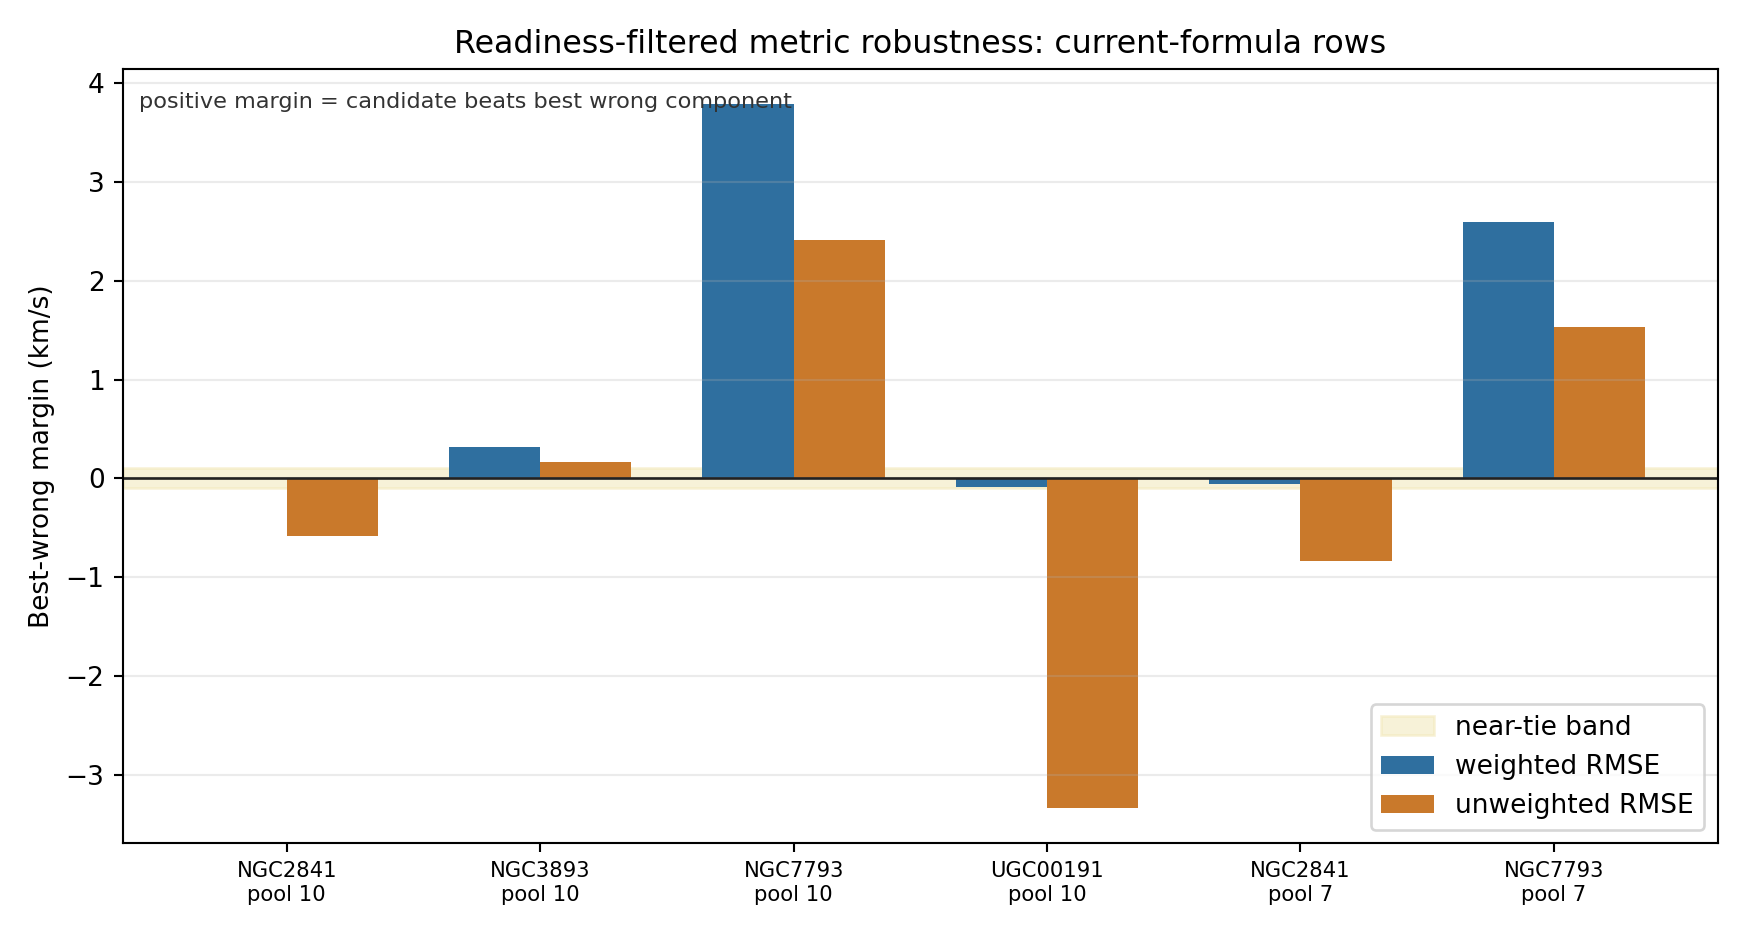
\includegraphics[width=0.92\linewidth]{figures/tcdr_readiness_filtered_metric_robustness.png}
\caption{\textbf{Readiness-filtered metric robustness.}  The figure shows the
best-wrong margin for the six current-formula rows allowed by the Paper8/Paper9
readiness ledger.  Positive values mean that the candidate formula beats the
best wrong-component control under the stated metric.  The strict best-wrong
count is \(3/6\) under both weighted and unweighted RMSE, but several weighted
near-tie rows weaken under unweighted RMSE.  This is retained as a robustness
diagnostic, not endpoint validation.}
\label{fig:readiness-metric-robustness}
\end{figure}

The mixed-route opening was then tested directly rather than assumed.  For the
four rows in which a source-visible secondary component explains the best-wrong
control, the source non-overlap condition closes: the relevant bar/ring
supports are source-side disjoint under the support-aware ledger.  However, a
64-shuffle formula-package control does not pass for any of the four rows at
the predeclared \(p\leq 0.10\) threshold.  The remaining two
\(K_{\rm obs}\) versus \(K_{\rm readout}\) rows are the NGC0024 broad-disk
cases.  A separate source-side review blocks their spiral readout relabel:
the broad family label contains disk/spiral structure, but the frozen source
ledger has bar/ring support, zero spiral component weight, and no source-native
spiral geometry.  The final route-closure ledger therefore leaves only the six
current-formula rows replay-ready and keeps 11/17 rows blocked: 5 source-gap
rows, 4 mixed-route shuffle-control failures, and 2 source-review-blocked
\(K_{\rm obs}\)/\(K_{\rm readout}\) relabels.  These negative results are
retained: source-visible secondary components or broad observed-family labels
are not, by themselves, enough to promote new endpoint kernels.
A final source-gap ledger inspects the 5 source-gap rows and finds that all are
competitive spiral controls outside the frozen source family, without
independent source-side spiral support.  They therefore remain source-acquisition
tasks rather than replay candidates.
We then performed a bounded external literature/source audit of these same
source-gap rows, recorded in
\path{scripts/build_tcdr_v4_source_gap_external_literature_audit.py}.  This
audit does not close the blocker.  UGC04499 gains an anti-spiral source-side
constraint: it appears in a late-type/bulgeless study as a featureless disk
without large-scale spiral structure \cite{DamasSegovia2012Bulgeless}.
UGC06917 remains a bar-dominated source route under the available S4G manifest
without an independent spiral/projection/history token.  UGC12732 has useful
non-bar caveats from star-formation morphology and global H\,I/kinematic
catalogues \cite{DiazGarcia2020SFbars,Murugeshan2020AngularMomentum}, but no
source-native spiral geometry or independent path/history token sufficient to
promote the competitive spiral control.  The route permission therefore remains
\texttt{keep\_source\_gap\_blocked} for all five source-gap rows.
The resulting post-external route-closure artifact,
\path{data/external/sparc_preflight/tcdr_v4_post_external_route_closure_local.csv},
keeps the same six current-formula rows replay-ready and leaves the other
eleven rows blocked: five source-gap rows after external audit, four mixed-route
shuffle-control failures, and two source-review-blocked
\(K_{\rm obs}\)/\(K_{\rm readout}\) relabels.
The final scoring-boundary summary,
\path{data/external/sparc_preflight/tcdr_v4_post_external_scoring_boundary_local.csv},
therefore treats only those six current-formula rows as score-bearing.  On that
permission-filtered subset, the weighted score beats the baryonic carrier and
the wrong-component mean in \(6/6\), while strict best-wrong survival remains
\(3/6\).  Under the unweighted RMSE robustness metric, wrong-component-mean
survival falls to \(4/6\) and best-wrong survival remains \(3/6\).  Blocked rows
carry no scoring claim in this summary.

\begin{figure}[H]
\centering
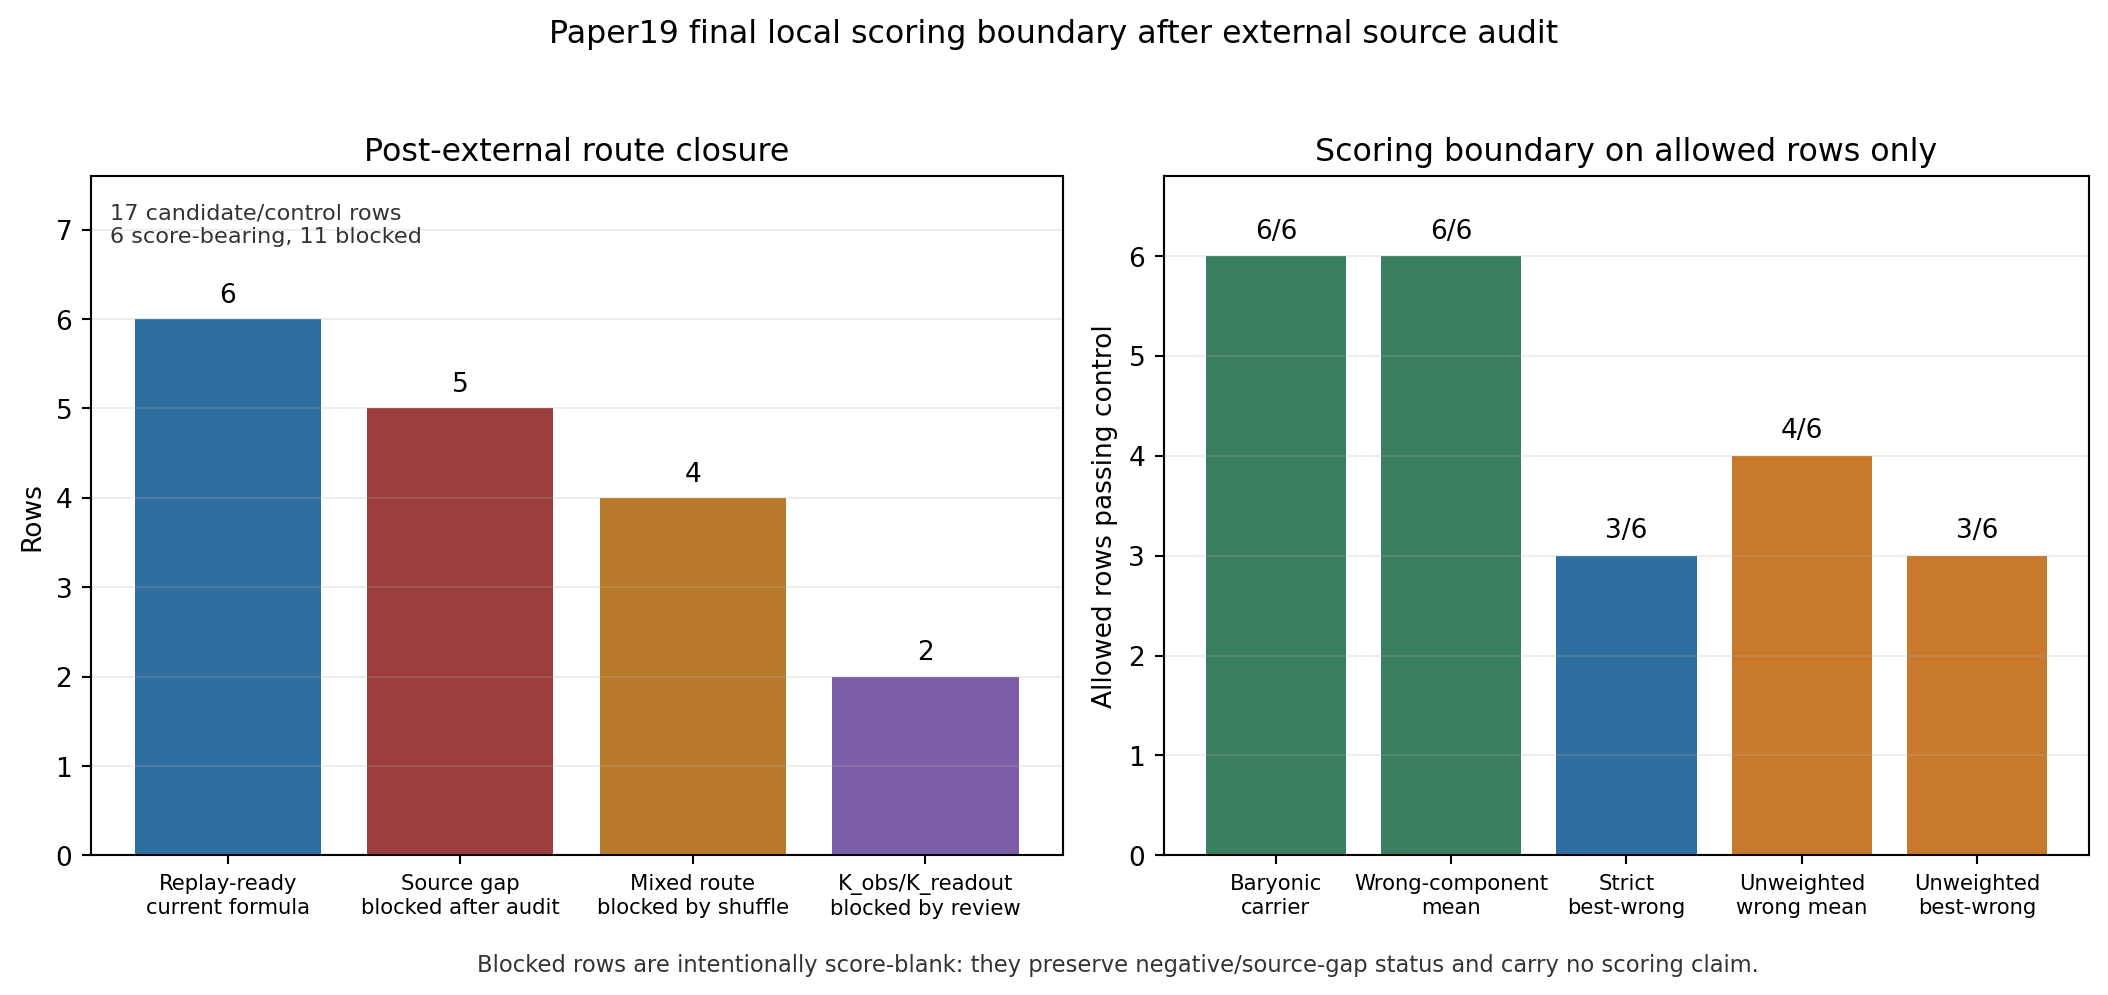
\includegraphics[width=0.94\linewidth]{figures/tcdr_post_external_scoring_boundary.png}
\caption{\textbf{Post-external scoring boundary.}  The left panel gives the
final route-closure ledger after the bounded external source audit.  Only the
six current-formula rows remain replay-ready; the other eleven rows are blocked
by source gaps, mixed-route shuffle controls, or source-review relabel blockers.
The right panel reports control survival only on those six allowed rows.
Blocked rows are intentionally score-blank and carry no scoring claim.  This is
a local diagnostic boundary, not population validation.}
\label{fig:post-external-scoring-boundary}
\end{figure}

\begin{sloppypar}
Finally, we ask whether the three strict best-wrong failures inside the
score-bearing subset can be upgraded into source-visible mixed routes.  The
diagnostic artifact
\path{data/external/sparc_preflight/tcdr_v4_allowed_best_wrong_failure_diagnostic_local.csv}
joins the six allowed rows to the frozen source-composition ledger.  It finds
zero source-visible best-wrong secondary components among the three strict
failures.  These rows are therefore not promoted to mixed kernels from the
endpoint score.  They remain near-tie or metric-sensitive control-pressure
diagnostics, and the next honest improvement path is additional residual-blind
source evidence rather than endpoint-driven kernel repair.
The corresponding source-acquisition worklist,
\path{data/external/sparc_preflight/tcdr_v4_allowed_failure_source_acquisition_worklist_local.csv},
contains three row-level requests across two galaxies, NGC2841 and UGC00191.
All three requests ask for independent spiral/path/history evidence and keep
both endpoint replay and kernel promotion set to \texttt{no}.  Thus the paper
does not convert the remaining best-wrong pressure into a new route; it records
exactly what source-side evidence would be needed before such a route could be
reviewed.
The first bounded external source-review artifact,
\path{data/external/sparc_preflight/tcdr_v4_allowed_failure_external_source_review_local.csv},
then separates source-side review from endpoint permission.  For NGC2841,
independent morphology/path evidence exists: ESA/Hubble identifies the object
as a flocculent spiral with short spiral arms \cite{ESAHubbleNGC2841}, and
Dragonfly reports an extended stellar disk with an outer warp
\cite{Zhang2018NGC2841Dragonfly}; the ring component remains independently
consistent with the molecular/ring morphology route already used in the source
ledger \cite{YoungScoville1982MolecularRings}.  This is enough to mark a future
NGC2841 spiral/path route as source-reviewable, but not enough to score it.  For
UGC00191, the source pass is weaker: the S4G outer-feature catalogue gives only
a tentative asymmetry flag for UGC 191 \cite{Laine2014S4GOuterFeatures}, and
the DensePak LSB study provides H$\alpha$/kinematic coverage without
source-native spiral geometry \cite{KuzioDeNaray2008LSBMassModels}.  Thus
UGC00191 remains a weak asymmetry/path review case, not a route-closing spiral
case.  Both rows keep endpoint replay and kernel promotion set to
\texttt{no}.
\end{sloppypar}

\begin{table}[H]
\centering
\scriptsize
\setlength{\tabcolsep}{3pt}
\begin{tabular}{L{0.19\linewidth}L{0.23\linewidth}L{0.15\linewidth}L{0.13\linewidth}L{0.18\linewidth}}
\toprule
Source & TCDR role & Source-label use & Endpoint use & Leakage guard\\
\midrule
SPARC sample table & sample metadata and control & conditional & no & no residual label rescue\\
SPARC mass models & baseline and endpoint component & no & yes & no family choice\\
SPARC Rotmod files & endpoint dynamics & no & yes & labels must already be frozen\\
S4G/IRSA & source-side morphology & yes & no & no rotation residual scoring\\
Galaxy Zoo & morphology crosscheck & yes & no & freeze before endpoint inspection\\
EDD/Cosmicflows & distance and environment control & conditional & conditional & no post-hoc tuning\\
\bottomrule
\end{tabular}
\caption{TCDR-v4 real-data source manifest v0.1.  This table is a protocol
artifact, not a data analysis.  It fixes which public data products are allowed
to define source-side labels and which are endpoint/baseline quantities.}
\label{tab:real-data-manifest}
\end{table}

\section{TCDR-v4 Real-Data Protocol Skeleton}

The TCDR-v4 protocol is the real-data-facing output of the package.  Its
recommended sequence is:
\begin{enumerate}
  \item nearby spiral galaxies with rotation curves and baryonic profiles;
  \item add source-side morphology and filament/environment variables;
  \item stack galaxy-galaxy lensing by morphology/environment class;
  \item compare null and timelike residuals where both are available;
  \item only then move to cluster lensing plus dynamics.
\end{enumerate}

The required controls include halo-family variation, cored versus cusped
comparison, baryonic mass-to-light marginalization, gas uncertainty, distance
and inclination uncertainty, non-circular motion flags, pressure support,
source redshift uncertainty, shear calibration, mass-sheet/projection effects,
neighbor catalogues, tidal indices, survey footprint controls, and
permutation controls within matched mass/morphology bins.

\section{Relationship to Existing Frameworks}

The TCDR protocol does not replace MOND, \(\Lambda\)CDM, or halo modeling.
MOND-like phenomenology can be an effective acceleration-scale relation
\cite{Milgrom1983}; halo models can fit broad gravitational phenomenology
\cite{Navarro1996,Burkert1995}; lensing and cluster systems provide strong
evidence that any serious model must account for null-probe mass mapping
\cite{Clowe2006,Mandelbaum2018}.  TCDR is a different diagnostic question:
after conventional modeling and controls, is there a residual component tied
to predeclared morphology, boundary, or null/time split variables?

If the answer is no, the TCDR branch fails for that dataset.  If the answer is
yes, the result is still only a candidate; it must survive independent data,
out-of-sample validation, and shared-parent covariance checks.

\section{Failure Modes}

The protocol is designed to fail.  Failure occurs if:
\begin{itemize}
  \item improved halo or baryonic modeling absorbs the residual;
  \item seed correlations vanish under permutation or matched-bin shuffling;
  \item the signal follows survey footprint, inclination, or selection bias;
  \item the apparent null/time split is dominated by ordinary lensing or
  dynamics systematics;
  \item out-of-sample validation fails.
\end{itemize}
These failures would not disprove Tau Core globally, but they would block the
TCDR dark-residual branch in the tested domain.

\section{Discussion}

The strongest result of this package is not the presence of high scores under
strong synthetic injection.  That is expected.  The useful result is the
combination of recovery under injected source-side structure and score-zero
behavior in the no-injection runs.  This provides a minimal audit grammar for
future data work.

The TCDR-v3 null/time split is especially important because it is more
specific than a generic residual-amplitude test.  It asks whether null probes
and timelike probes separate in a way that follows source-side structure.  A
real-data version would be scientifically interesting only if the split
survived lensing, dynamics, baryonic, halo, and survey controls.

\section{Conclusion}

Paper 19 promotes the Photon-C dark residual package into a reproducible
synthetic paper.  The package defines a careful test ladder:
\begin{align*}
  \hbox{source-side seeds}
  &\rightarrow \hbox{standard controls}\\
  &\rightarrow \hbox{Tau-extended recovery}\\
  &\rightarrow \hbox{permutation/null tests}\\
  &\rightarrow \hbox{real-data TCDR-v4 protocol}.
\end{align*}
The current status is
\[
  \textsc{Controlled Synthetic Photon-C Dark Residual Protocol}.
\]
It is not observational evidence and not physical validation.  It is a
structured way to ask, in future real data, whether dark-sector residuals
contain a morphology-seeded null/time component that standard controls do not
absorb.

\bibliographystyle{plain}
\bibliography{refs}

\end{document}
